\documentclass{jimis-en}
\pdfoutput=1 %forces arXiv/HAL to compile with PDFLaTeX

% Packages
\usepackage{array}
\usepackage{pgfplots}
\usepackage{graphicx}

% header
\title{Identifying European Sustainable Mega-city Regions with Multi-dimensional Network Percolation}
% Endogenous urban regions as an optimal compromise between economic integration and greenhouse gases emissions
% A multi-dimensional percolation approach to characterize sustainable mega-city regions



\author[1,2,3,*]{Juste RAIMBAULT}
\affil[1]{UPS CNRS 3611 ISC-PIF, France} 
\affil[2]{CASA, UCL, UK}
\affil[3]{UMR CNRS 8504 G{\'e}ographie-cit{\'e}s}
 
% corresponding author with his/her email
\corrauthor{juste.raimbault@polytechnique.edu}

%% Information provided by JIMIS:
%ISSN
% DOI 
\doi{10.18713/JIMIS-ddmmyy-v-a}{}
% reviewing process: first date = submission, second date = acceptance 
\review{Month-in-letters Day Year}{Month-in-letters Day Year}
% Volume and Year of the issue
\publication{N}{YYYY}

%% Information provided by the Editors:
% Issue Title 
\issue{Title of the interdisciplinary issue}
% List of k Editors
\editors{First-name-$1$ Family-name-$1$, First-name-$2$ Family-name-$2$, First-name-$k$ Family-name-$k$...}

\begin{document}

\maketitle

\abstract{Territorial structure significantly conditions the sustainability of human settlements. Recent forms of urbanization, in particular integrated mega-city regions, may imply different patterns of economic and transportation flows and thus exhibit various performances regarding different indicators of sustainability. This paper proposes to reconstruct endogenous urban regions from the bottom-up using network percolation, in a multi-dimensional way to take into account both urban form (spatial distribution of population) and urban function (properties of transportation networks). Variable parametrizations allows to consider patterns of optimization for two stylized contradictory sustainability indicators (economic performance and greenhouse gases emissions). This suggests a customizable spatial design of policies to develop sustainable territories.}

\keywords{Road network; multilayer percolation; mega-city region}

\section{Introduction}

\strut
\vspace{-4ex}


% Morphologies of networks and territories
% - intro : LGV ? Avignon : travaux Claire ! - truc avec les Papes ? 
% https://www.persee.fr/doc/anami_0003-4398_1985_num_97_172_2228_t1_0446_0000_3
% https://www.persee.fr/doc/mefr_0223-5110_1984_num_96_1_2762

% -> visu OSM : see Metropolitan region ; plus positioning of Avignon ; Q of sustainibility ?


% les formes des établissements humains peuvent se percevoir a differentes echelles et selon differentes dimensions. Elle font partie de notre vie courante, a ces mutiples echelles, et pourtant nous sont si etrangeres. Afin d'introduire notre sujet, je propose ici une image familière pour bien d'entre vous qui fréquentent cette région.
% La metropole etendue de la region marseilleise ne se limite pas a l'aspect administratif d'aix marseille, mais englobe bien avignon et la ciotat, voire manosque, des lors que l'on prend un certain recul geographique.
% il n'aura pas manque aux eoils attentifs que ce recul est d'autant plus une abstraction, puisque nous ne represnetons ici uniquement les reseaux routiers, qui s'averent deja etre un proxy suffisant pour estrapoler une densite d'activités humaines.
% Cette presentation s'axera ainsi sur la morphologie des reseaux et des territories et sur leurs relations.
%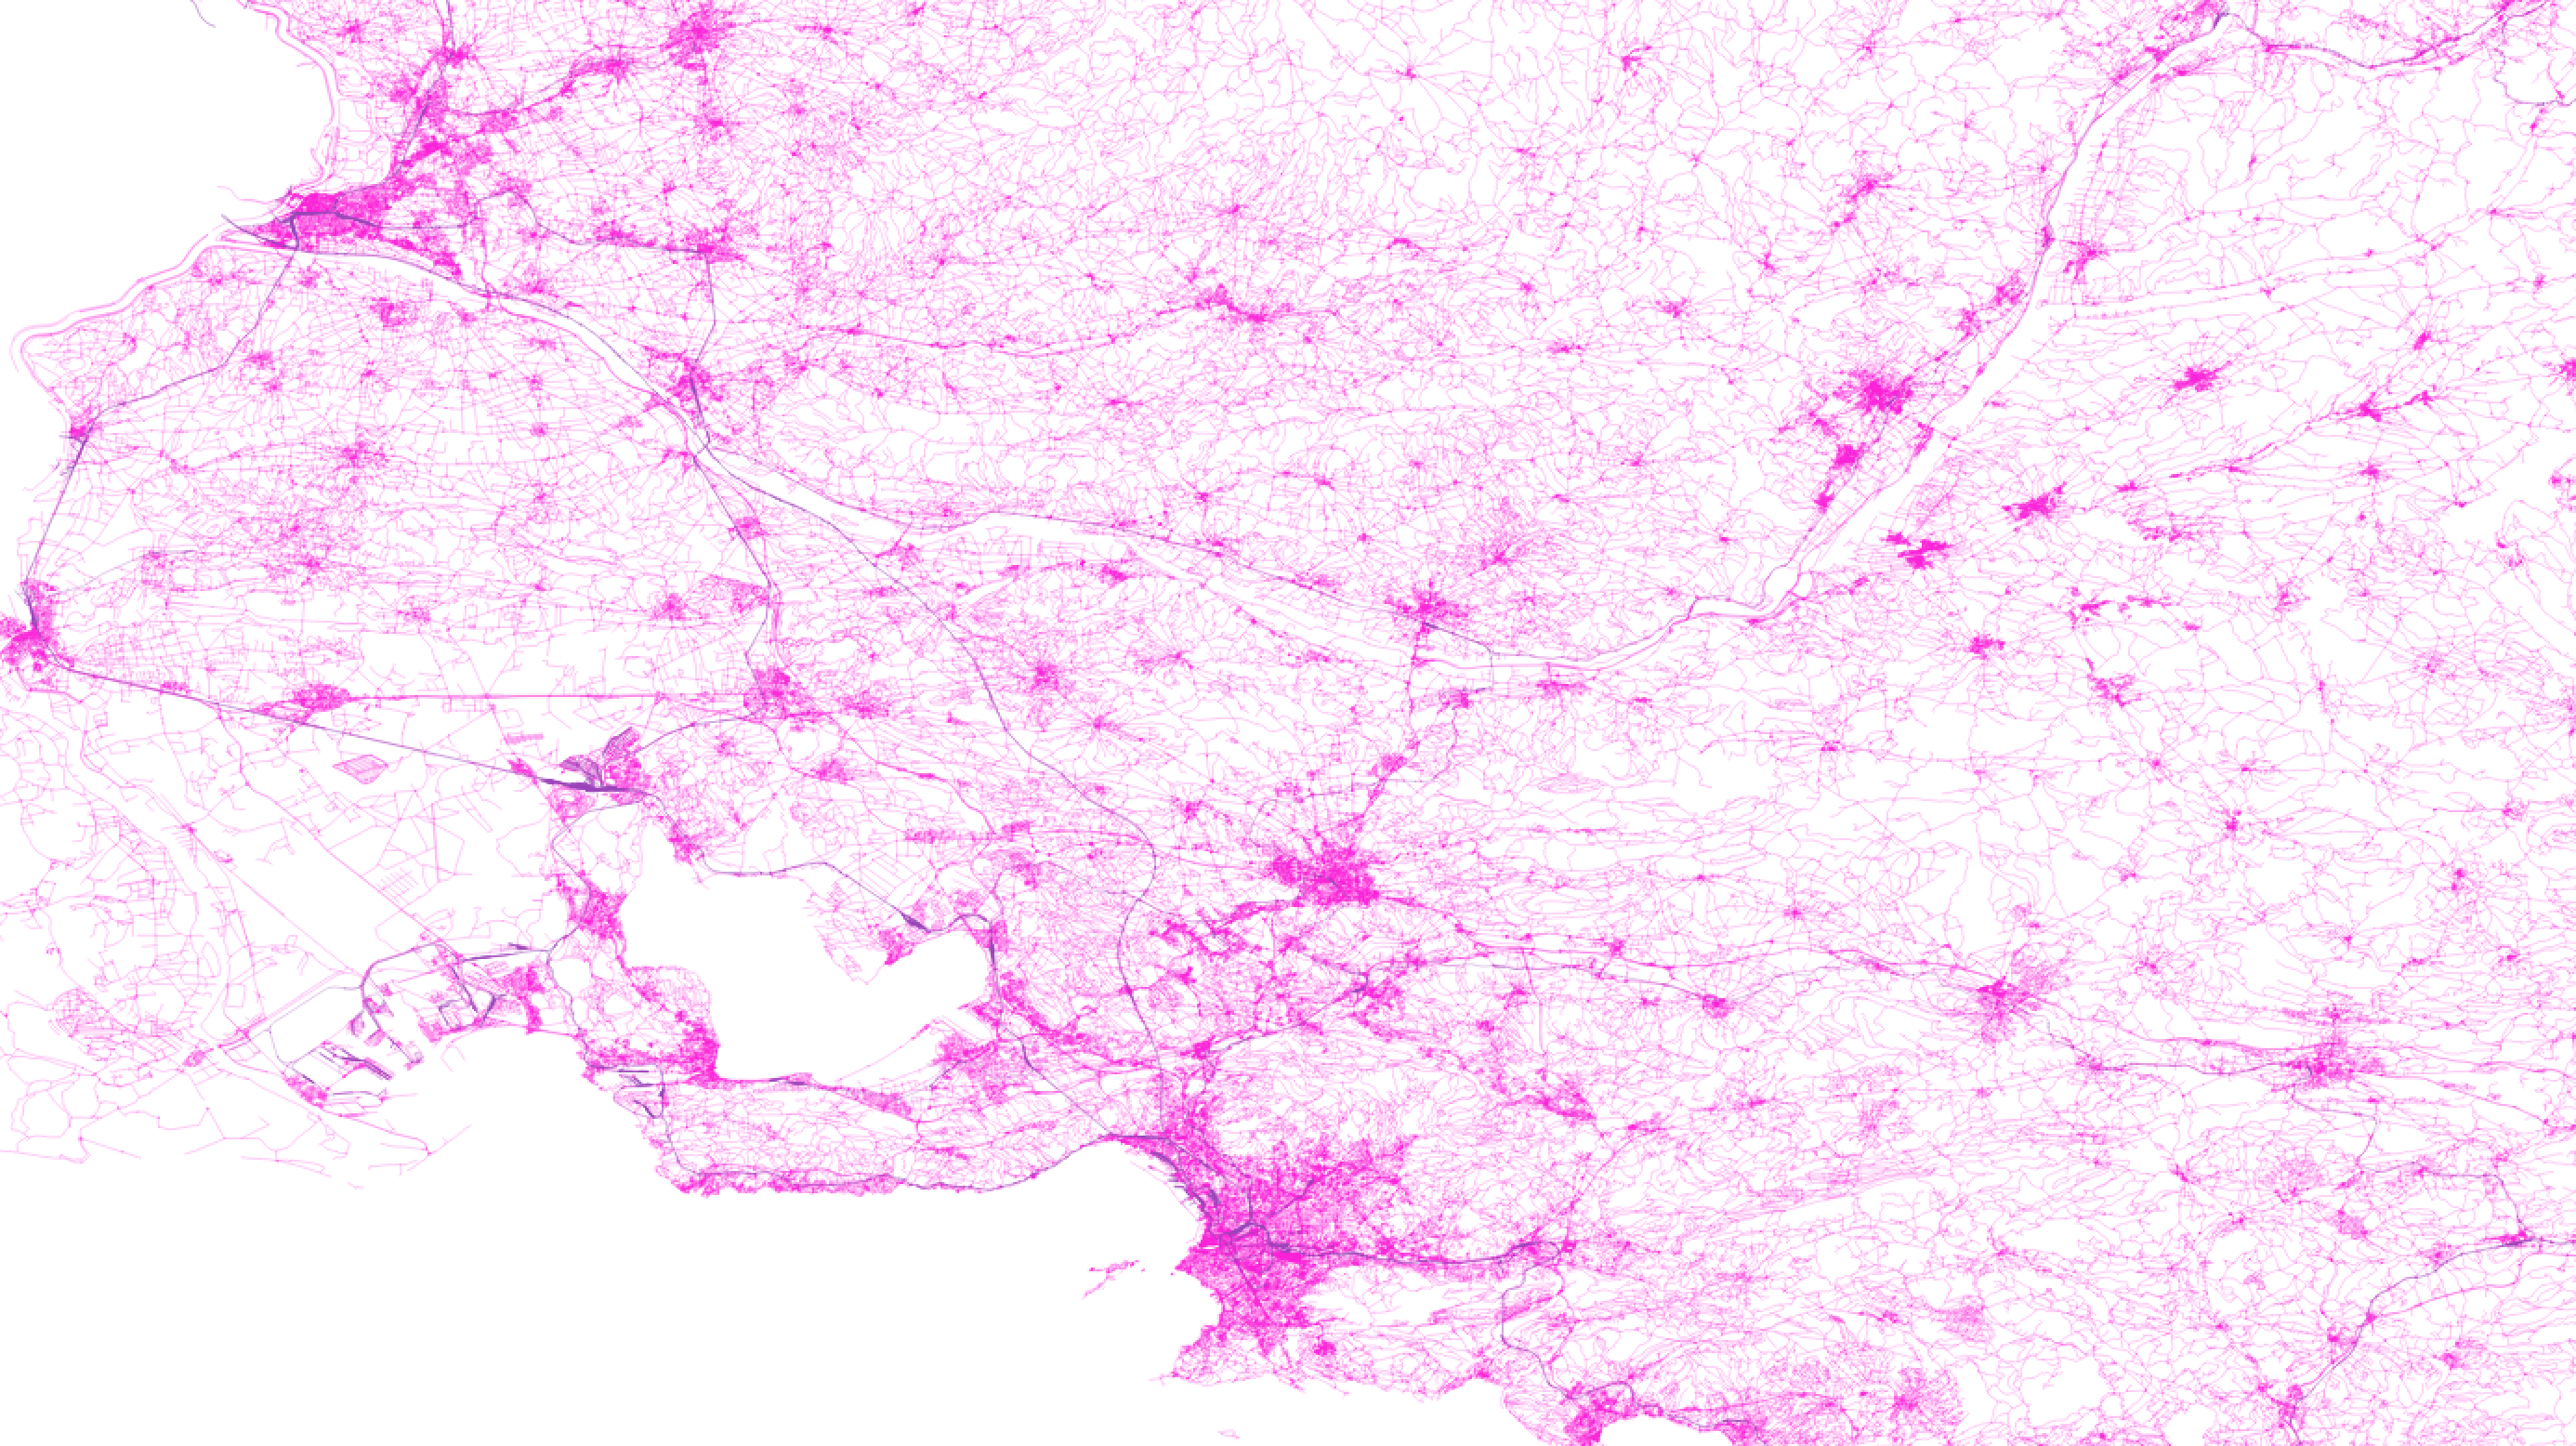
\includegraphics[width=1.2\textwidth]{figures/roadssouth.png}
%\textit{Source: OpenStreetMap}

The structure of road networks both translates its past growth dynamics and has a significant impact on the sustainability of territories it irrigates. Diverse methods to characterize the structure of spatial networks, and more particularly road networks, have been developed in that context.


% here extracts from Claire's work
% Lagesse, C., Bordin, P., & Douady, S. (2015). A spatial multi-scale object to analyze road networks. Network Science, 3(1), 156-181. -> nice picture Avignon

% La caracterisation des reseaux routiers, par exemples en termes de classification et dindicateurs topoliques, est liee a differents enjeux qui incluent la comprehnsion des dynamiques ppasses par la contingence de ces artefacts, amis qussi des questions futues liees a la soutenabilité des territoires qui'ils irriguent.
% les developpements recents, issus d'efforts interdispclinaires, incluent par exmeple ce travail de Claire Lagesse applique a la ville que v ous reconnaissaez bien, pour la definition de nouveau object a la pertineence thematique plus grande que les seuls entites des bases de donnes sans ontologie propre. (ex perso ballade avignon hier : vraie coherence thematique de l'objet "Way")

%\textit{Multiple dimensions to characterize road networks}
%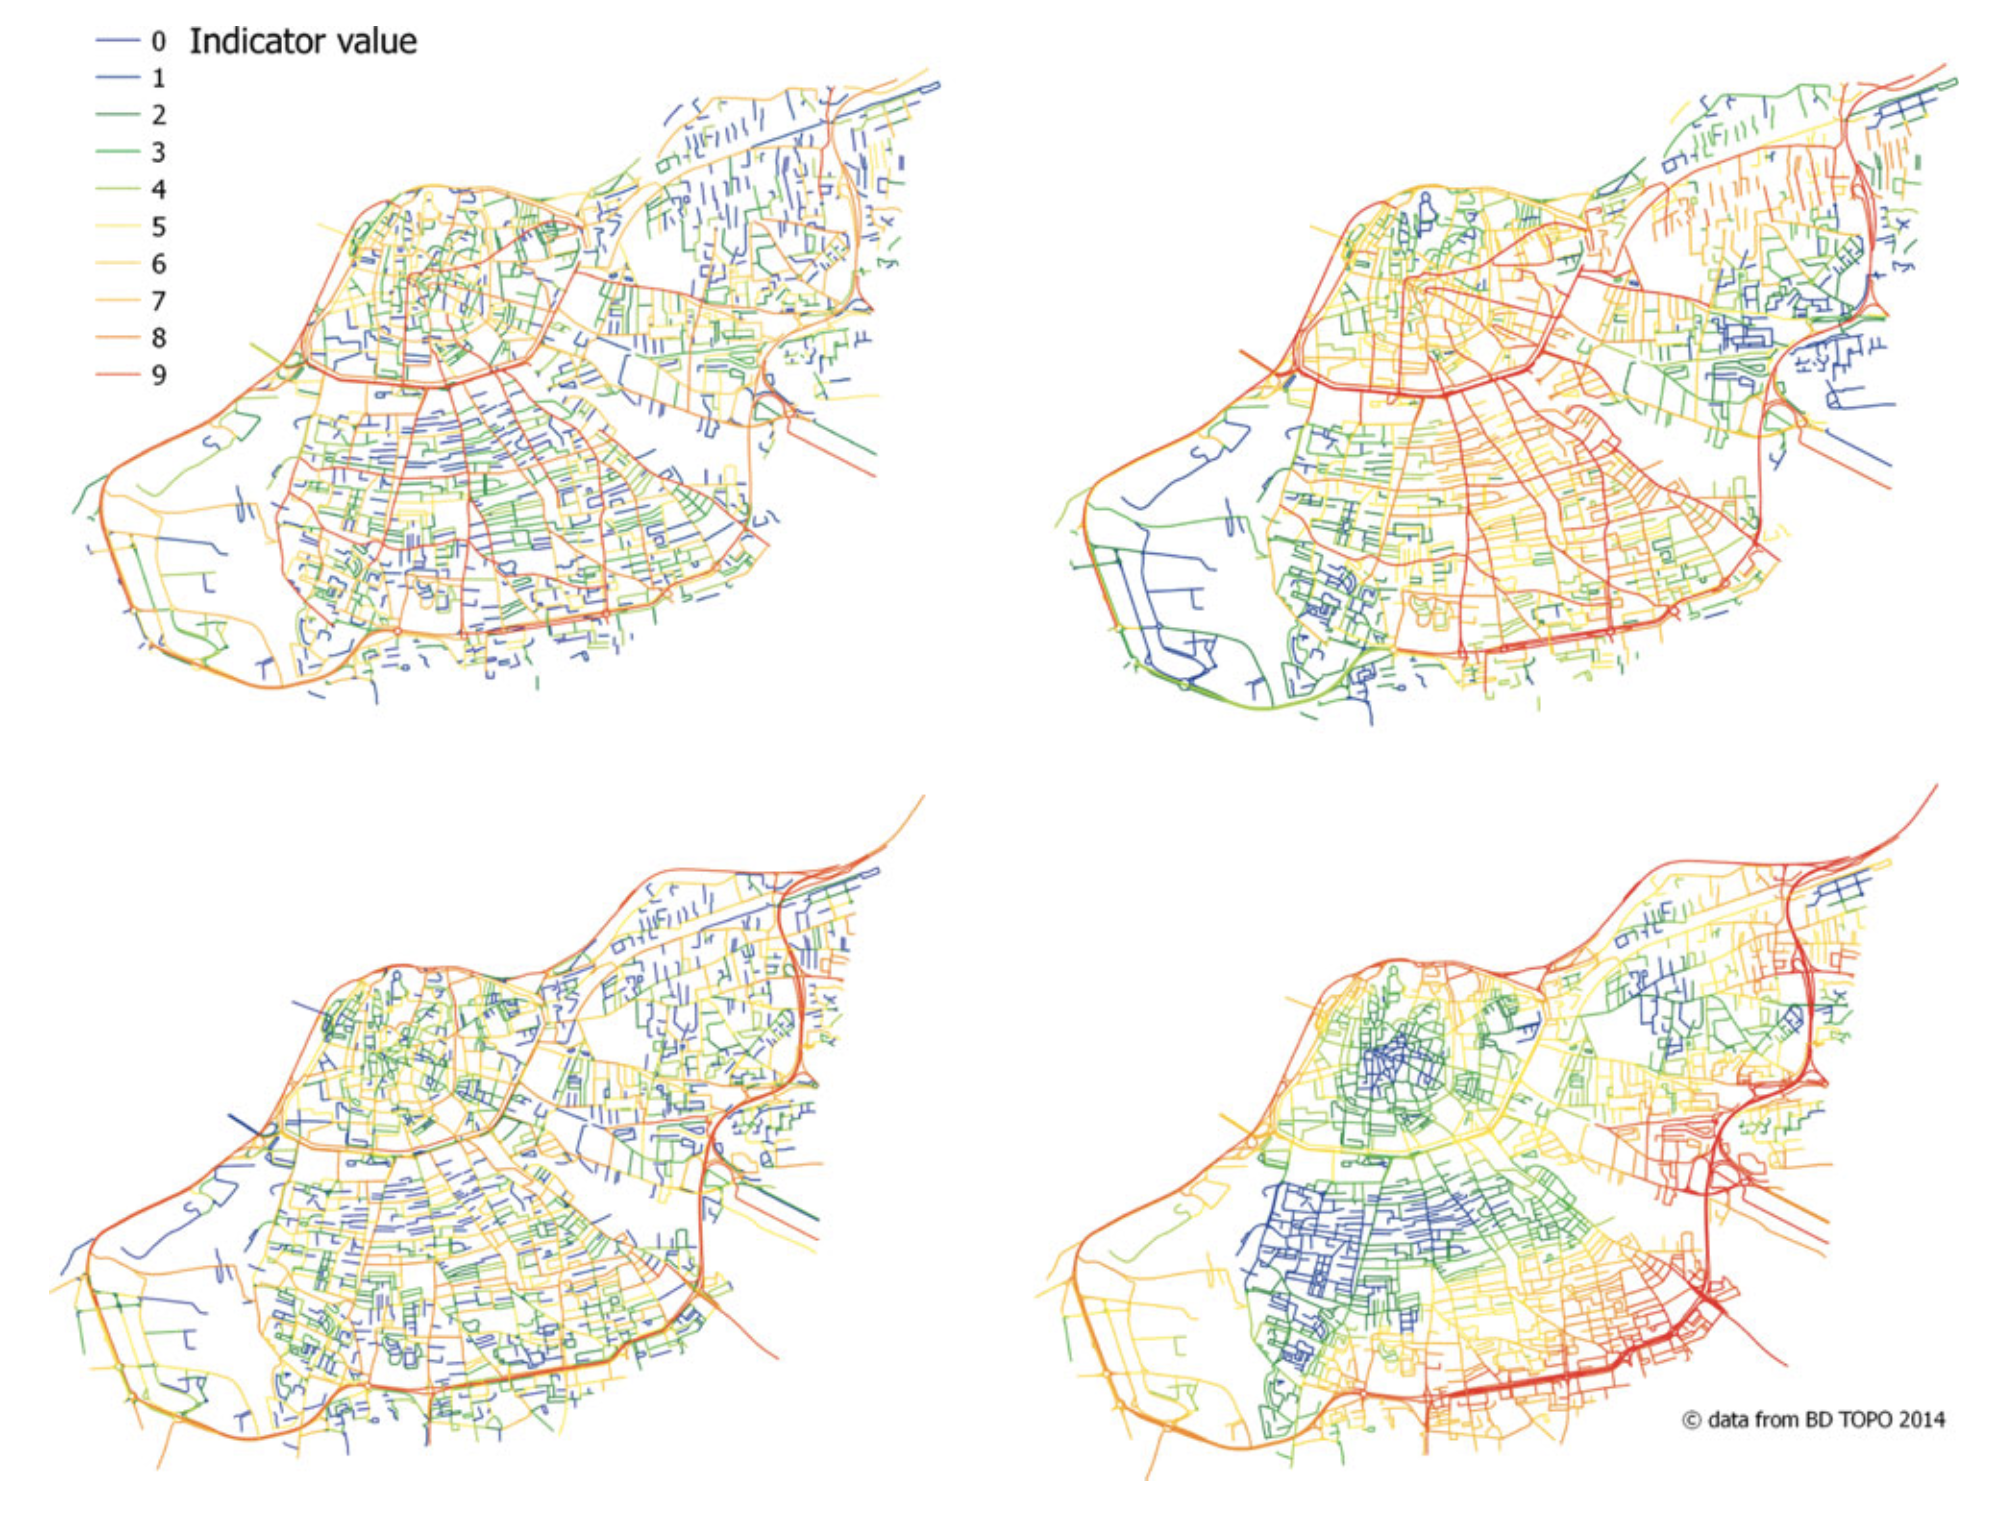
\includegraphics[width=\textwidth,height=0.7\textheight]{figures/avignon_claire.png}

%Lagesse, C., Bordin, P., \& Douady, S. (2015). A spatial multi-scale object to analyze road networks. Network Science, 3(1), 156-181. \cite{lagesse2015spatial}




A method to characterize topologies of these spatial networks is network percolation. Such approaches have been applied to the modeling of urban growth \citep{makse1998modeling} and to the analysis of street networks for example to extract endogenous urban regions \citep{arcaute2016cities} or to characterize the spatial morphology of point patterns \cite{huynh2018characterisation}.


%Network percolation
% A method to characterize topologies of these spatial networks is network percolation. Such approaches have been applied to the modeling of urban growth \citep{makse1998modeling} and to the analysis of street networks for example to extract endogenous urban regions \citep{arcaute2016cities} or to characterize the spatial morphology of point patterns \cite{huynh2018characterisation}.

% from monodimensional to multidimensional

% similar to 
%Cottineau, C., Finance, O., Hatna, E., Arcaute, E., & Batty, M. (2018). Defining urban clusters to detect agglomeration economies. Environment and Planning B: Urban Analytics and City Science, 2399808318755146.

% 

% parmi ces outils, la percolation a ete applique recemment aux reseaux routiers.
% en phyique, ce phenomene designe la traversee d'un milieu plus ou omins poreux par un fluide, et par exetnsion les processus pour l'attendre. En pariculier, nous l'entendrons au sens d'une occupation progressice des sites / connections des noeus d'un reseau, jusqu'a un etat critique ou l'ensemble de ceux-ci sont connectés (percolation threshold). [probailite de perco p_c]
% en particulier ppour letude des viulles
% des travaux relaticement anciens ont propose un phenomene de percolation locale correlation pour modeliser l'etalement urbain.
% plus recemment, et plsu proches des travaux des physiciens, une determination endoganee des regions urbaines a etet proposee par l'equipe du acvs en appliquant une heuristqiue de percolation aux reseaux routiers.
% ces methodes peuvent egalement servier a effecteur des statistqieus spatiales.
% nous porposons ici d;'etendre ces methodes en prenant en compte differentes dimensions urbaines, de la meme maniere que cottineau et al combine densite de population et flux de commuting pour definir les regoins urbaines.

%\textbf{Network percolation: } \textit{progressive occupation/connection of nodes of a network} \cite{callaway2000network}

%Application to the study of cities:

%\begin{itemize}
%	\item modeling urban growth \cite{makse1998modeling}
%	\item endeogenous determination of regions \cite{arcaute2016cities}
%	\item characterization of spatial point patterns \cite{huynh2018characterisation}
%\end{itemize}
%\textit{Towards complementary dimensions to condition road network percolation}
%$\rightarrow$ similar to \cite{cottineau2018defining} to define urban areas





% necessity of multi-dimensional percolation

Existing heuristics however generally focus on a single morphological dimension of networks, and leave out the functional properties of urban systems \citep{burger2012form}.

This paper addresses such a gap by introducing a multi-dimensional percolation heuristic.

%Multidimensional percolation

% Existing heuristics however generally focus on a single morphological dimension of networks, and leave out the functional properties of urban systems \citep{burger2012form}.

% - why the relation between form and function, aka pop and network in our view is crucial
% - take into account in percolation
% - potential application : endogenous sustainable urban entities

% notre approceh reponde a la question ouverte du lien entre ofrme et fonction da`ns les systemes urbaine ;  et par ailleurs se base sur les interatcions entre reseaux te territoires poour fournire un proy de ce lien.
% nous propospns ainsi d'explorer une heuristique multi-dimensionnelle de la percolation qui prend en compte morplholohie urbaine et yopologie dy reseau routier ; nous l'appliquon pour caracterisere endogenement les regions urbaines.
% [rq : deux niveau de reseuax dans notree apporche : (mais en. fait comme souvent en geo ; ) le physique, et le abstraot que l'on construite a partir d'entites spatiales.

%$\rightarrow$ Need to combine morphological and functional dimensions of cities \cite{burger2012form}

%$\rightarrow$ Interactions between networks and territories to capture the link between form and function \cite{raimbault2018caracterisation}; potential application to sustainability of urban systems

% research question

%\textbf{Research objective : } \textit{Investigate a multi-dimensional percolation of territorial networks taking into account urban morphology and road network topology; endogenous characterization of urban regions.}




We percolate the population density layer with a network characteristic layer, that we test among number of edges, number of vertices, cyclomatic number and euclidian efficiency, which capture functional properties especially for the two last.



\section{Methods}



\subsection{Multi-dimensional percolation}


Given discrete spatial fields, site percolation is operated between two cells given a threshold parameter for each dimension and a distance threshold. This heuristic is similar to multilayer network percolation \cite{boccaletti2014structure}.

% decrivons a presons de neniere stylisee l'algorithme utilise.
% le processus de peroclation initrial est deterministe, base sur la distance, met est prochess des random eulidian networks evoque hier par Alain Franc : si deux neouds sont a une distance d'un rayon critique r_0, ceux ci sont connectes par un lien.
% nous ajoutons alors sur chaque couche du reaseu un seul de peroclation qui determine si le neod peut etre prus en compte dqns le reseau de la couhce.
% par conjonction des contraintes, nous obtenus un reseau a unique couche dans laquelle simplement els composantes connexes donnent les clusters perfcolés.


%%%%%%%%%%%%%%%%%%%%
\begin{figure*}[ht] 
%\resizebox{10cm}{7cm}
  {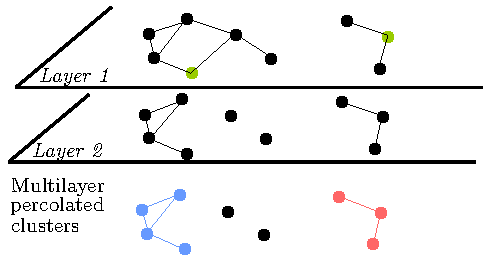
\includegraphics[width=\linewidth]{figures/principle.pdf}}
  \centering
  \label{fig:method}
  \caption{Schematic representation of the multi-dimensional network percolation heuristic.}
\end{figure*}
%%%%%%%%%%%%%%%%%%%%


%\textbf{Parameters: } percolation radius $r_0$, percolation thresholds $\theta_i$ for each layer




\subsection{Empirical data}


We apply the heuristic to urban morphology and road network topology measures in Europe. More precisely, a grid with resolution 50km of population density morphology indicators and road network topology indicators, has been computed on spatial moving windows for all European Union by \cite{raimbault2018urban}.


% Precisons a ppresent les objets geographiques a partir  desqueles nous allons construire le reseau.
% nous rappelns que nous cherchons a combiner prorpiete des territoires, que nous approximerons tres simplement par la districbution spatiale de la population, et propriete des reseaux routiers, que nous approximerons par des indicateirs topollogiques locaux.
% ces differentes caracteristqiues ont ete calucles, dans le cadre de ce travail de modelisation a l'echelle mesocscopique de la coevolution entre reseaux et cilles, sur les feentres glissantes de taille 50km poru l'ensemble de l'europe.
% nous en donnons ici l'illustration dans le cas de la France
% [several infos on different regimes etc]

%\textit{Territorial indicators computed for Europe by \cite{raimbault2018urban}}

% here add maps to better visualize the spatial fields

%\medskip

%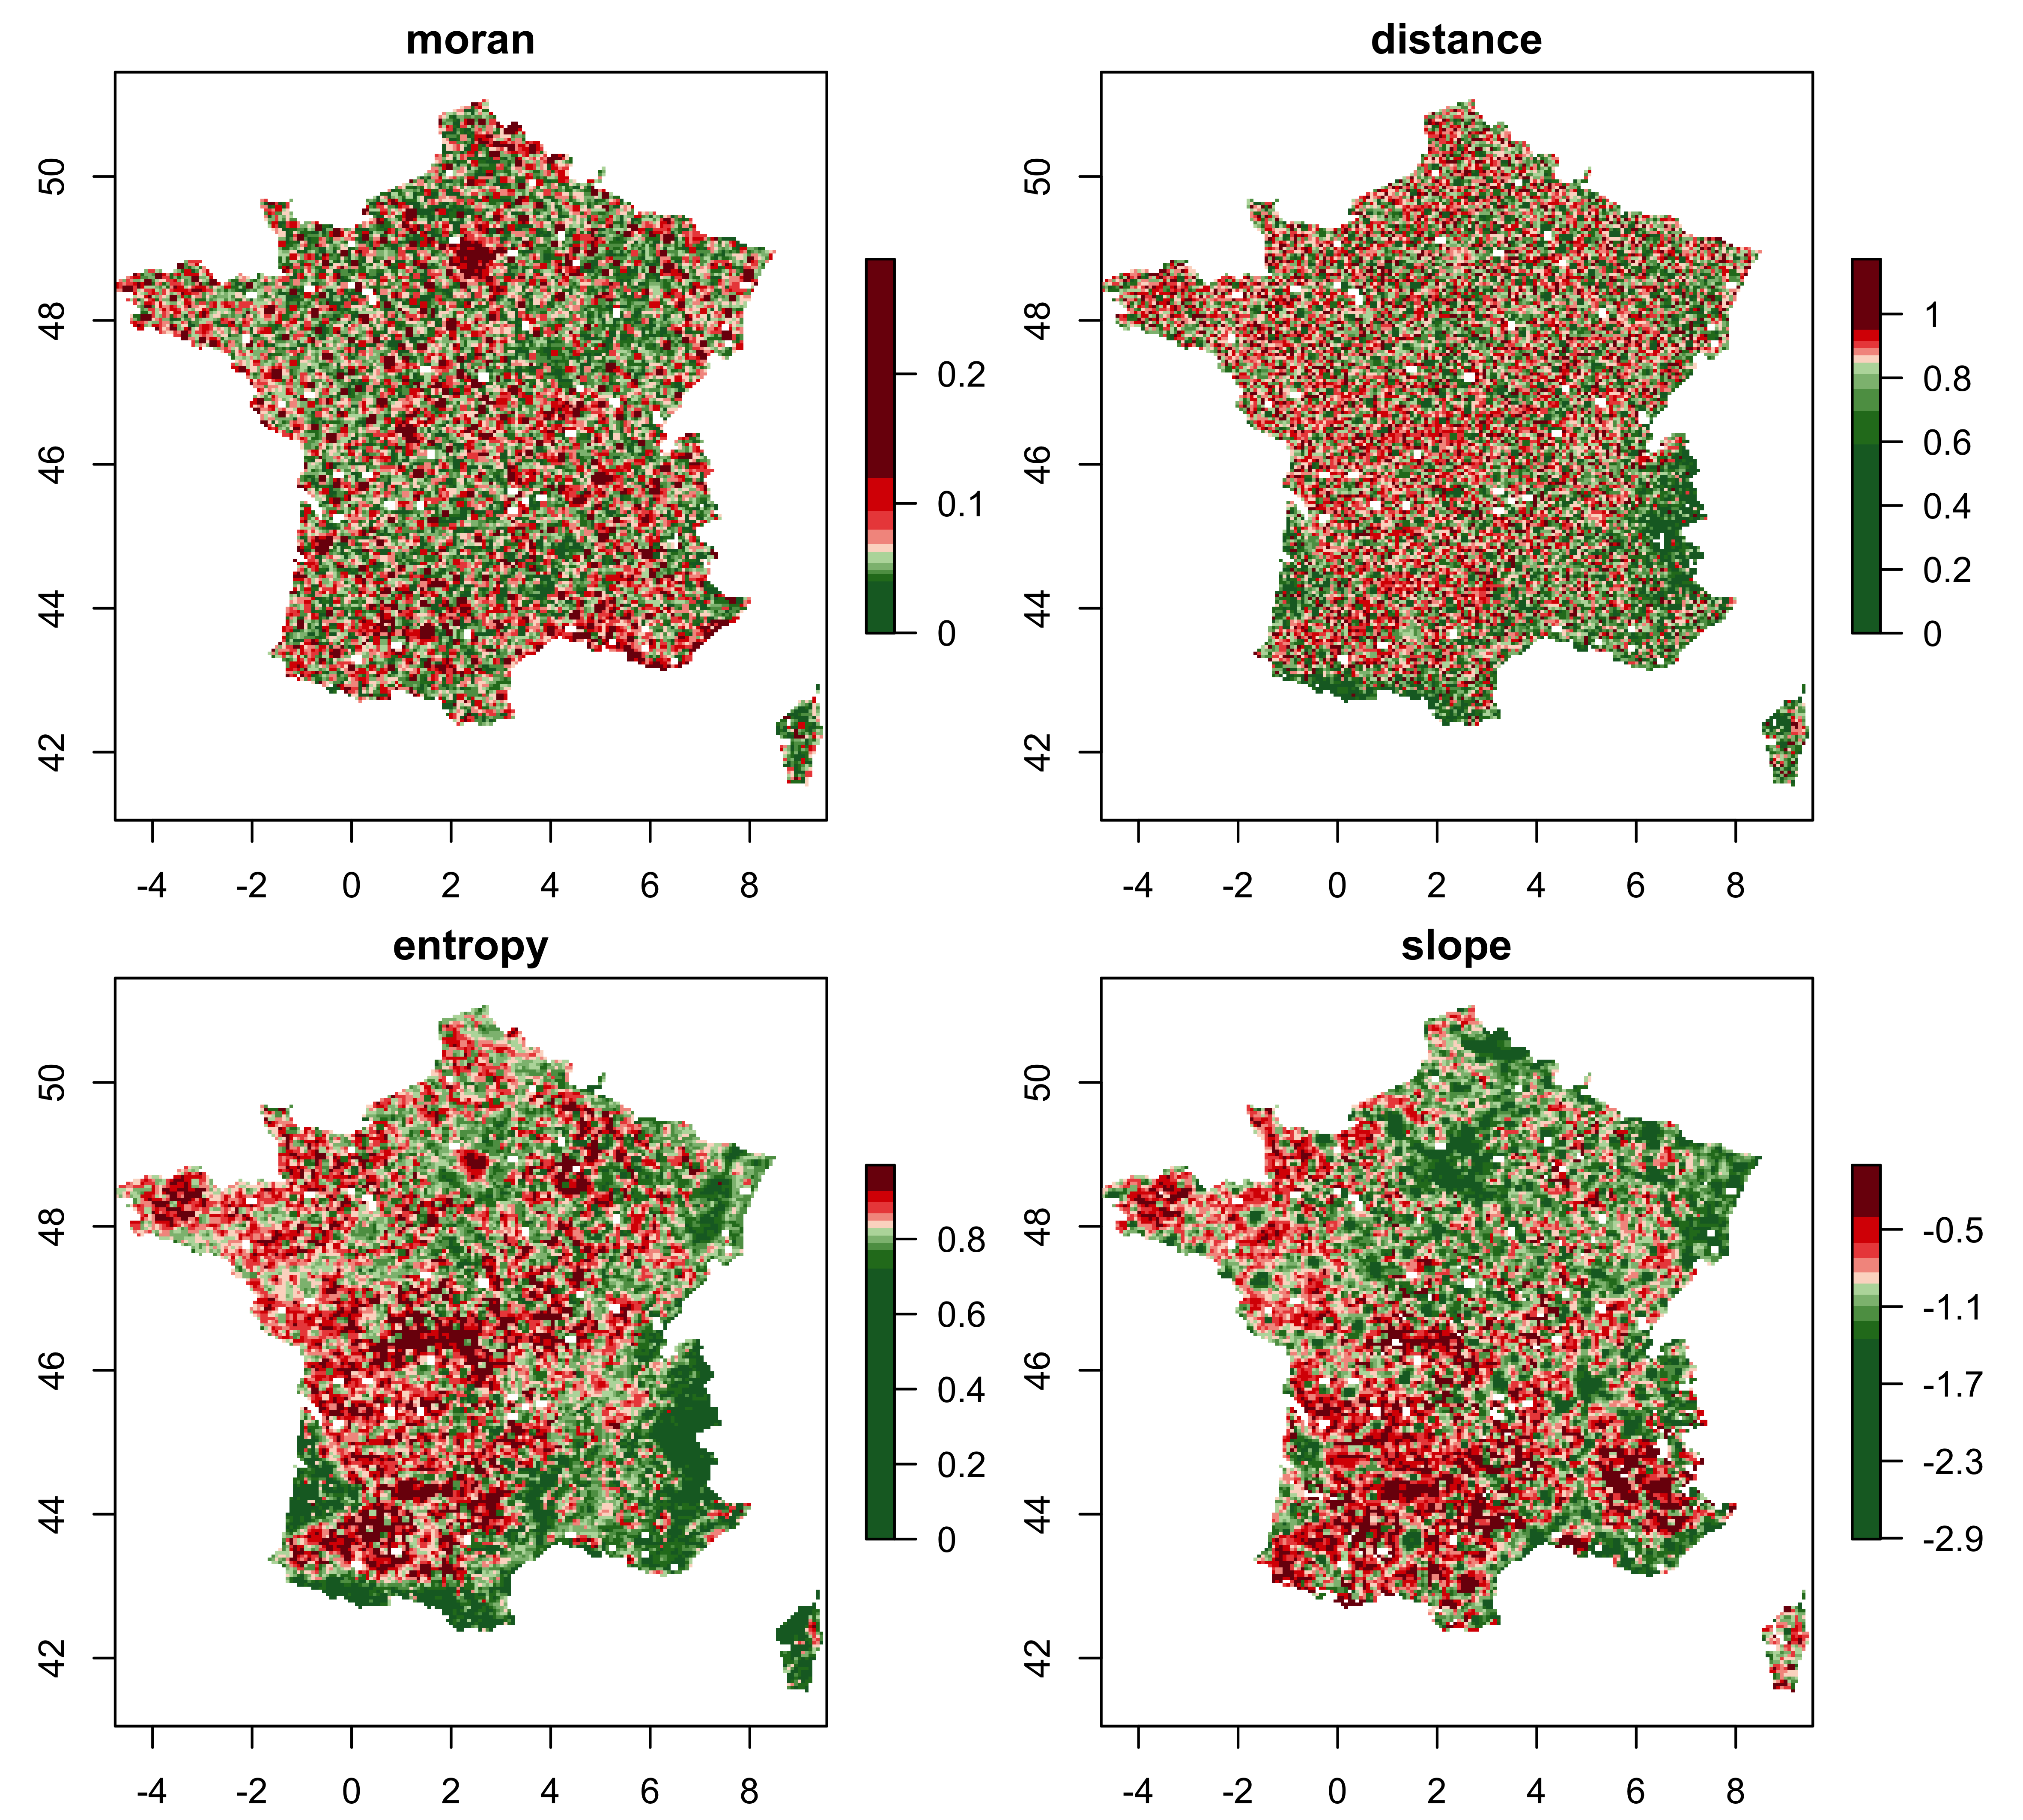
\includegraphics[width=0.49\textwidth]{figures/indics_morpho_discrquantiles.png}
%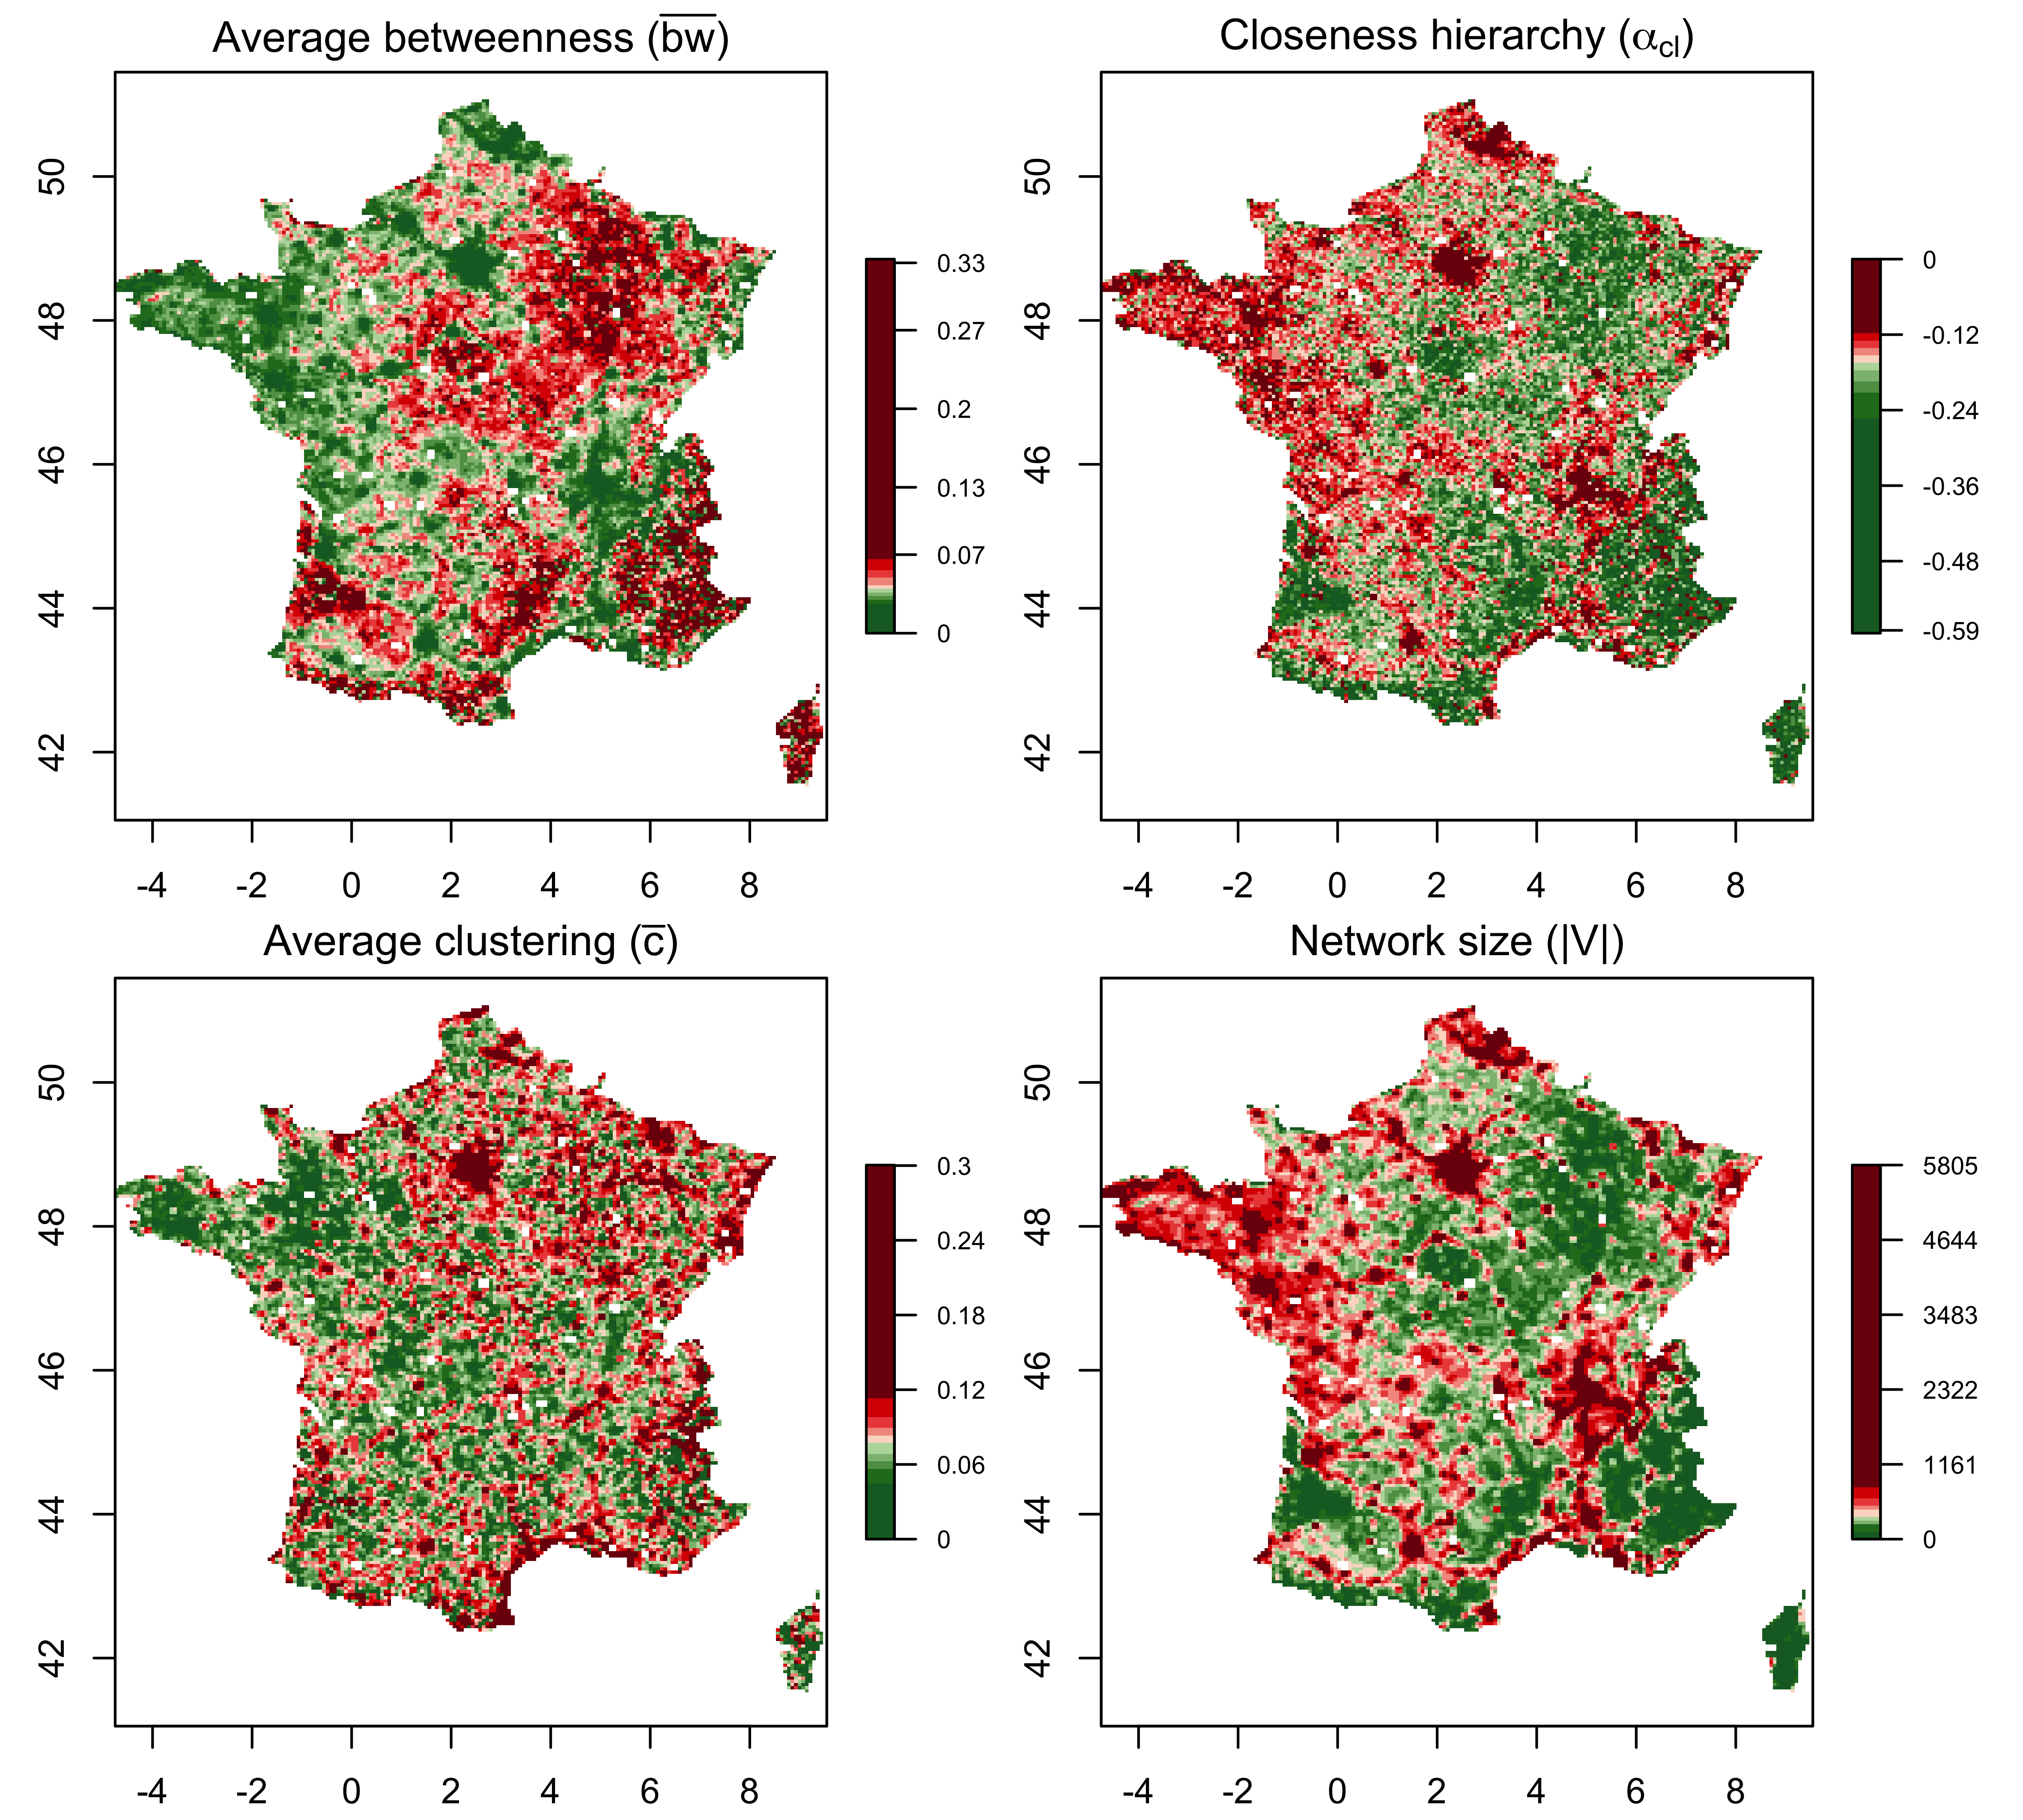
\includegraphics[width=0.49\textwidth]{figures/indics_network_en_areasize100_offset50_factor0_5.png}

%\textbf{Population distribution morphology} and \textbf{Network topology} (betweenness, closeness, clustering, efficiency, \ldots) computed on 50km spatial windows (Eurostat density grid and OpenStreetMap)





\subsection{Sustainability indicators}


We use this endogenous definition of regional urban systems produced by the percolation algorithm to evaluate their sustainability, in terms of conflicting objectives of economic integration and greenhouse gases emissions. The definition of sustainability, or sustainable development, is by essence multi-dimensional \citep{viguie2012trade}. Its characterization as quantitative indicators is even more subject to numerous degrees of freedom. We work here with two stylized indicators for two conflicting dimensions, as a proof-of-concept.


The EDGAR database \citep{janssens2017edgar} (version 4.3.2) is used for local estimates of greenhouse gases emissions.


% explain indicators : convex hull.

Applying a gravity model to each region, we estimate abstract transportation flows within each and extrapolate emissions by coupling with the Edgar emission database \citep{janssens2017edgar} and economic activities with a scaling law of population.  More precisely, greenhouse gases emissions derived from economic and transportation flows are estimated with the following expression 

\begin{equation}
\phi_{ij} = \left(\frac{v_i v_j}{(\sum_k v_k)^2}\right)^\gamma \cdot \exp\left(\frac{-d_{ij}}{d_0}\right)
\end{equation}

where $v_k$ are either effective local GHG emissions or population. Indeed, the economic activity follows relatively well scaling laws of populations \cite{bettencourt2007growth}, the exponent being dependant on the activity and the definition of areas on which it is estimated~\citep{cottineau2017diverse}.


The sum of all flows within the geographical span of the cluster (that we approximate as the convex Hull envelope of its points), allows us to approximate the cumulated potential emissions and economic activity.




\section{Results}

\subsection{Implementation}


%Network construction

%We percolate the population density layer with a network characteristic layer, that we test among number of edges, number of vertices, cyclomatic number and euclidian efficiency, which capture functional properties especially for the two last.

% a partir de ces deux couches nous considerosn d'un [art la densite de population, d'autre part des proxus pour la densite ou perdormance du reseau ; avce les paramteres associes.
% la logique geographique derriere cela est liee a la premiere loi de Tobler : deux lieus proches etc  ; ajoute a la logique de la masse (loi de gravite), mais selon different aspects du reseau (car difficile de savoir quelle dimenion a priori jouera le role "equivalent" d'une densite de population : autant laisser libre et explorer plutot que de fixer arbitrairemenbt - maxime d'un computational scientist converti, bien sur.
% en pratqiuem nous contruison le reseau correspondant et isolns ses composantes connexes.
% descirption du plan d'explericence.

%\textbf{Two layers: } population density (threshold $\theta_P$) and network characteristics (threshold $\theta_N$) taken among \{Number of edges, Number of vertices, Cyclomatic number $\mu$, Euclidian efficiency $v$ \}; percolated with a radius $r_0$

% banos2012towards

%\textbf{Rationale: } \textit{two locations will be in relation if they are close, have a high population density and given network characteristics.}

% note : euclperf should be minimized whereas other maximized : issue ?

%\textbf{Implementation: } construction of a single layer spatial network given the condition on the two layers and distances, from the 5km resolution indicators spatial field; extraction of connected components.

In practice, the analysis is implemented using R and the igraph package. The network is constructed by superposing the population density layer with the network layer.

%\textbf{Experience plan: } grid sampling for $r_0,\theta_P,\theta_N$ and network variables; additional gravity potential parameters $\gamma,d_0$ (detailed after)

The experience plan is a full grid, for parameters $r_0$, $\theta_P$, $\theta_N$ and the network variable considered.


%$\rightarrow$ 4800 parameter points
%We systematically explore the clusters obtained for 840 parameter configurations. 

% + explain openmole -> later in potential developments





We systematically explore the clusters obtained for 4800 parameter configurations.





\subsection{Extracting endogenous mega-city regions}

Maps reveal that most configurations resemble the actual distribution of European mega-city regions, which are functionally integrated polycentric urban areas \citep{hall2006polycentric}. These are here defined endogenously from the bottom-up.

% les rsultats sont particulierement interessantm puiqaue ceratines valuers de apremtres menest a des configurations connues par lkes geographesm celles des mega-cities regions
% [rq : affirnation arbitraire iuci car pas evidence-based, il faudrait comp systematique etc , le probeleme vcest que meme pas de liste avec consensus sur l'obejct, comme soubent en geo>...]
% du coup "visuellemtn" randstad, rehinrhuhrm, rehinmainm London, Paris, Manchester Leeds,




% note : forgot r_0 in figs
%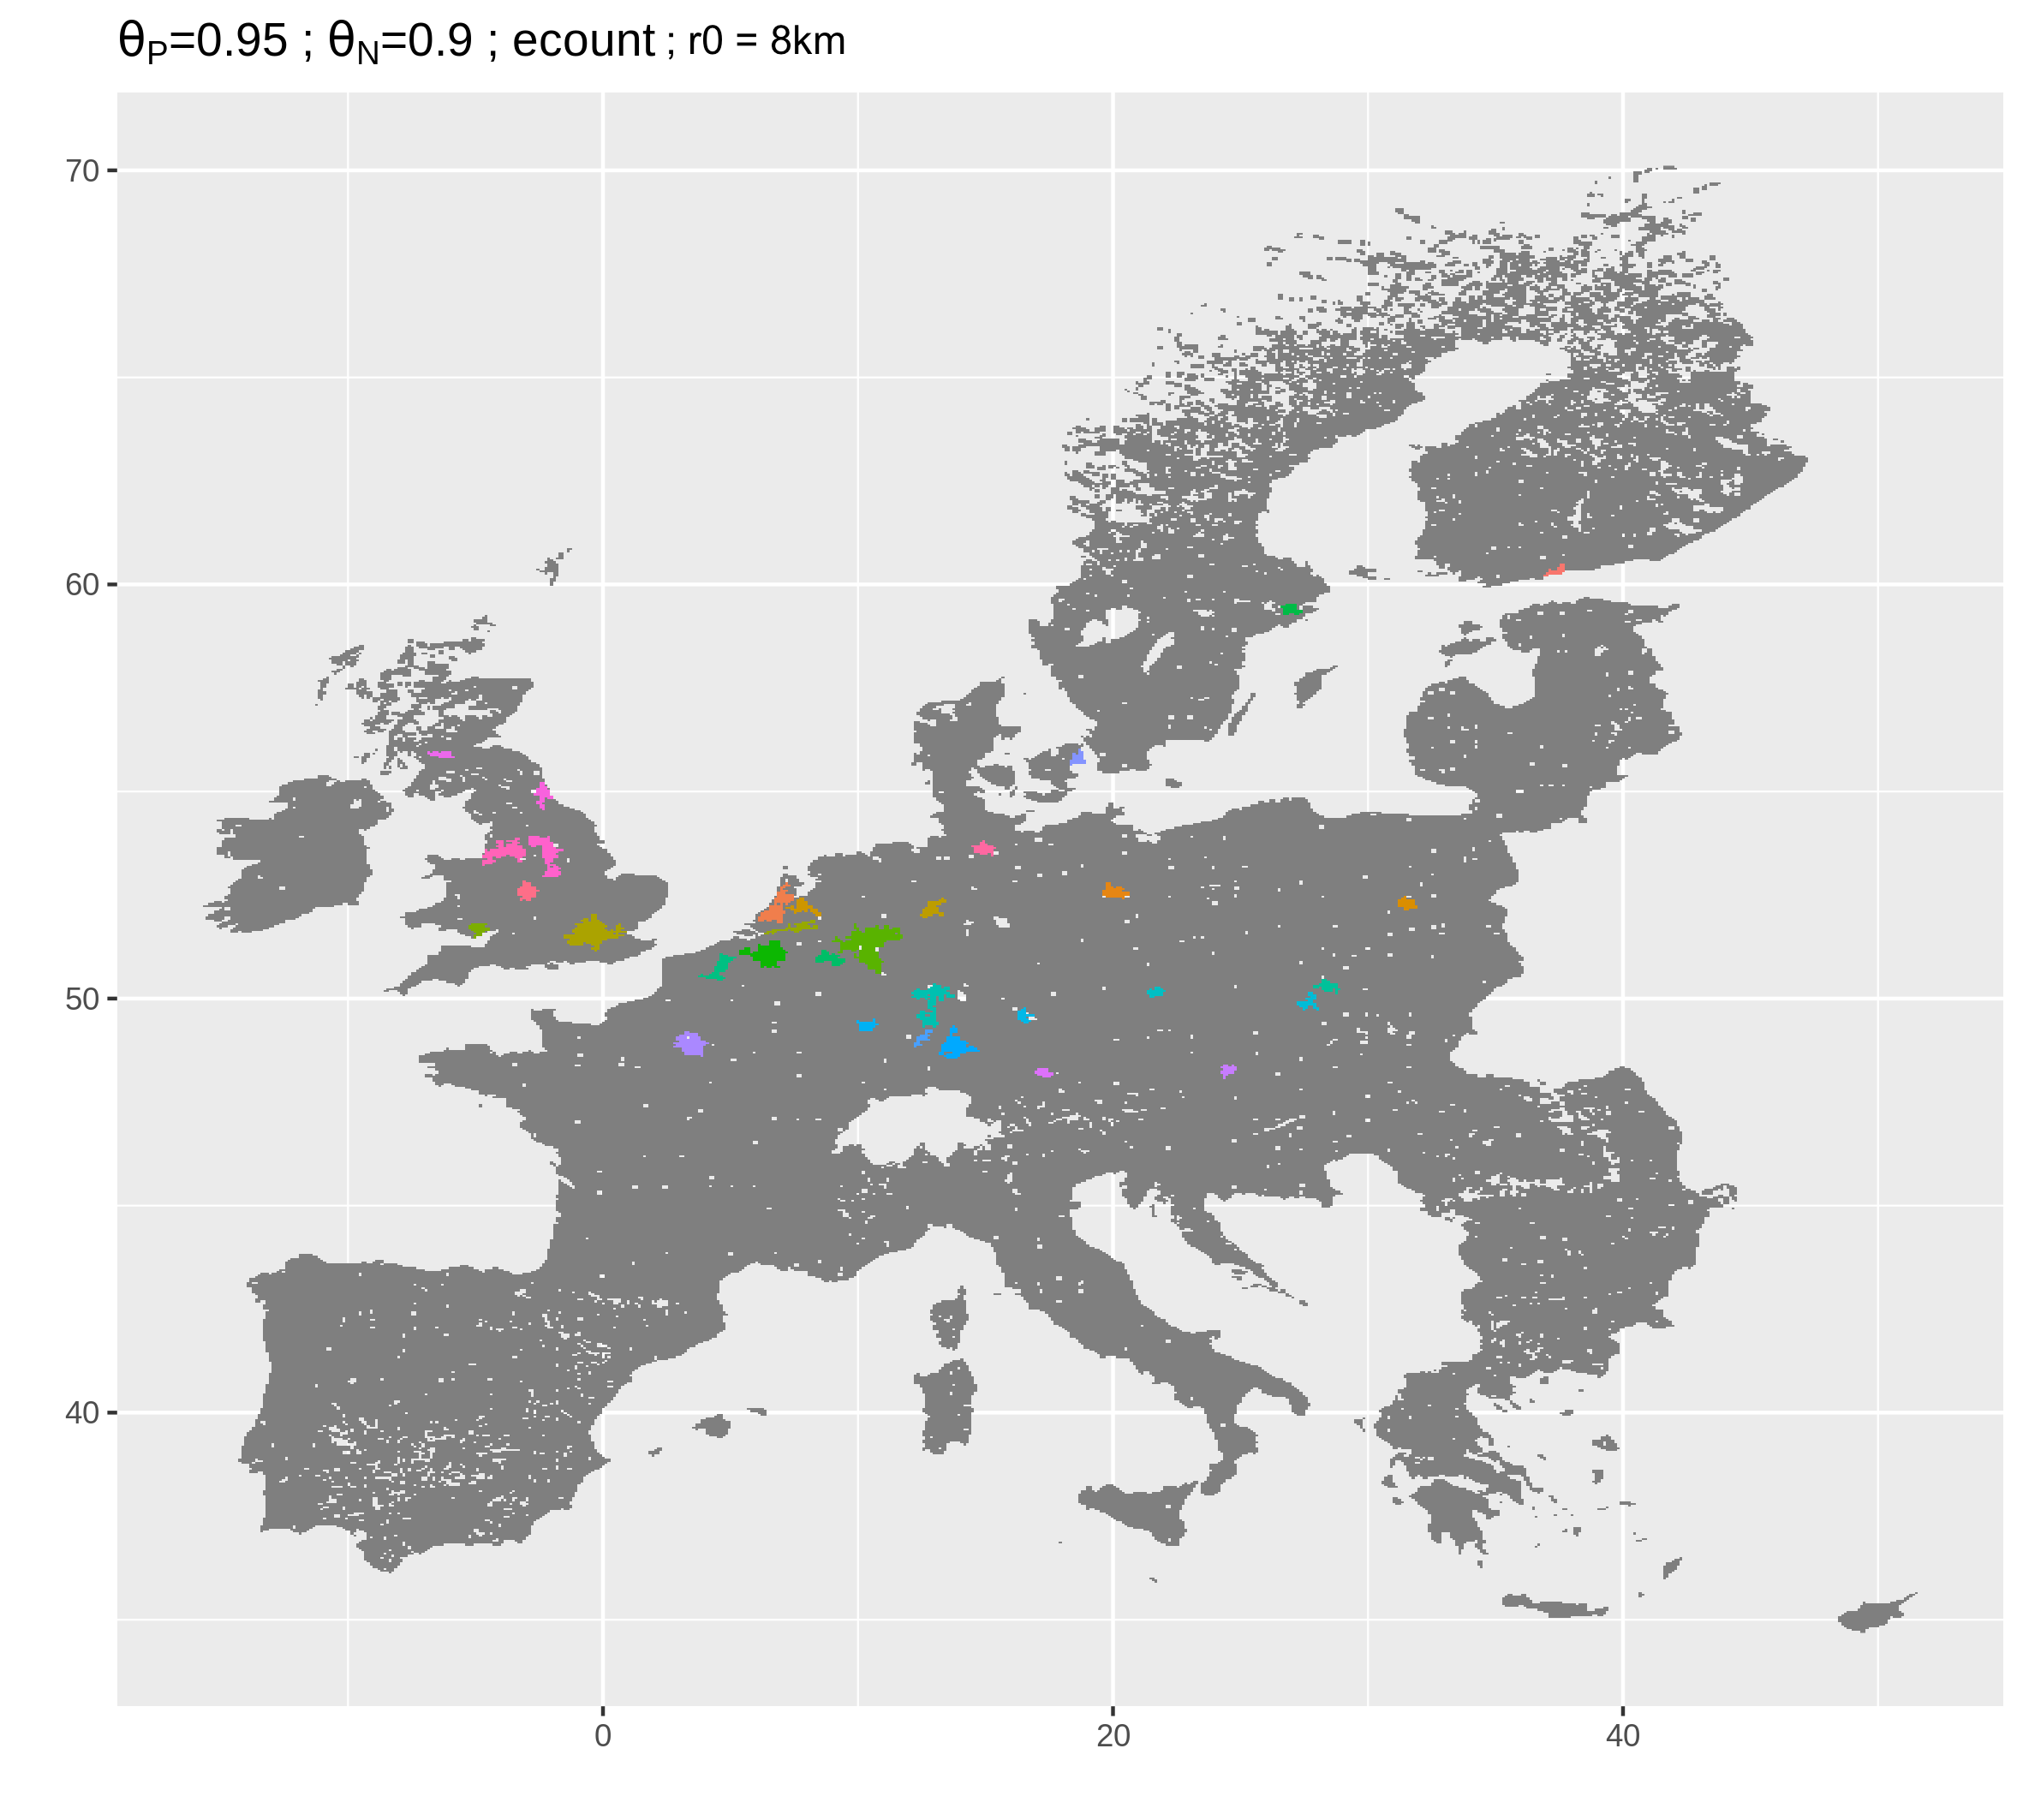
\includegraphics[width=\textwidth,height=0.9\textheight]{figures/totalPop4183694_00056402_ecount850_radius8000.png}

%Different endogenous morphologies

% TODO for the paper : check effect of adding network threshold : methodo info on multilayer percol in itself


%%%%%%%%%%%%%%%%%%%%
\begin{figure*}[ht] 
%\resizebox{10cm}{7cm}
  {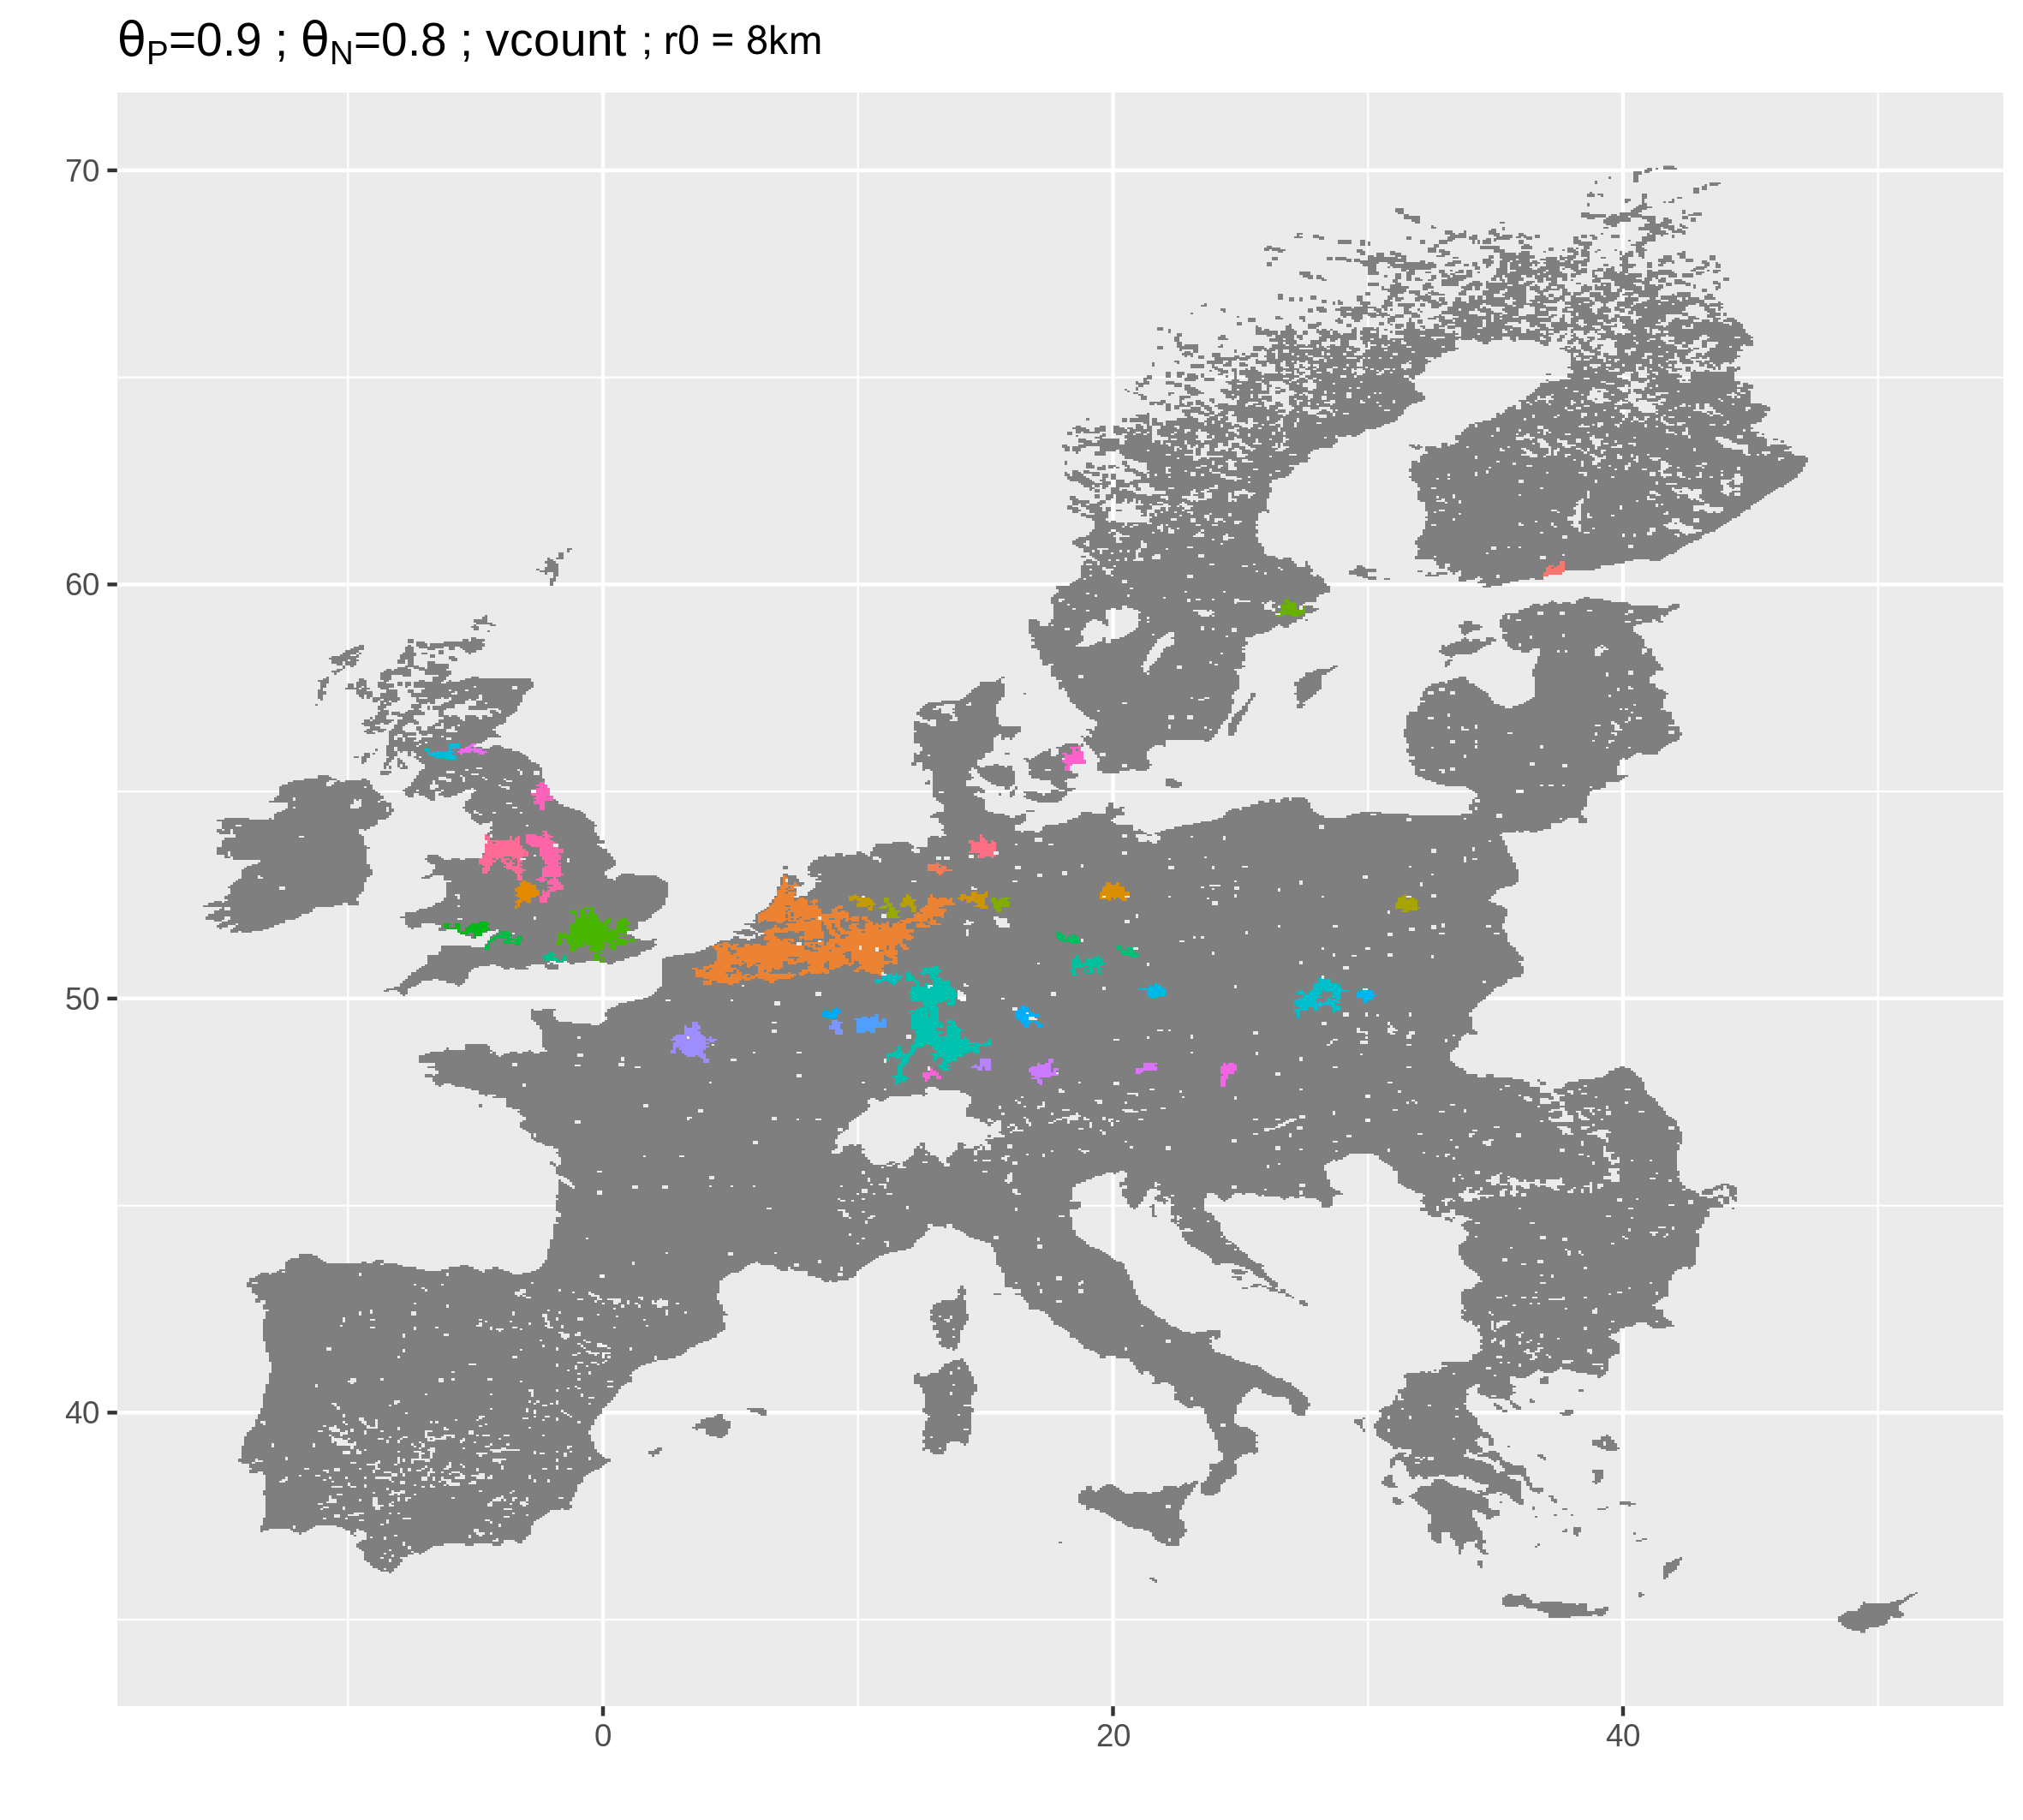
\includegraphics[width=0.49\linewidth]{figures/totalPop2219780_36719597_vcount378_radius8000.png}}
  {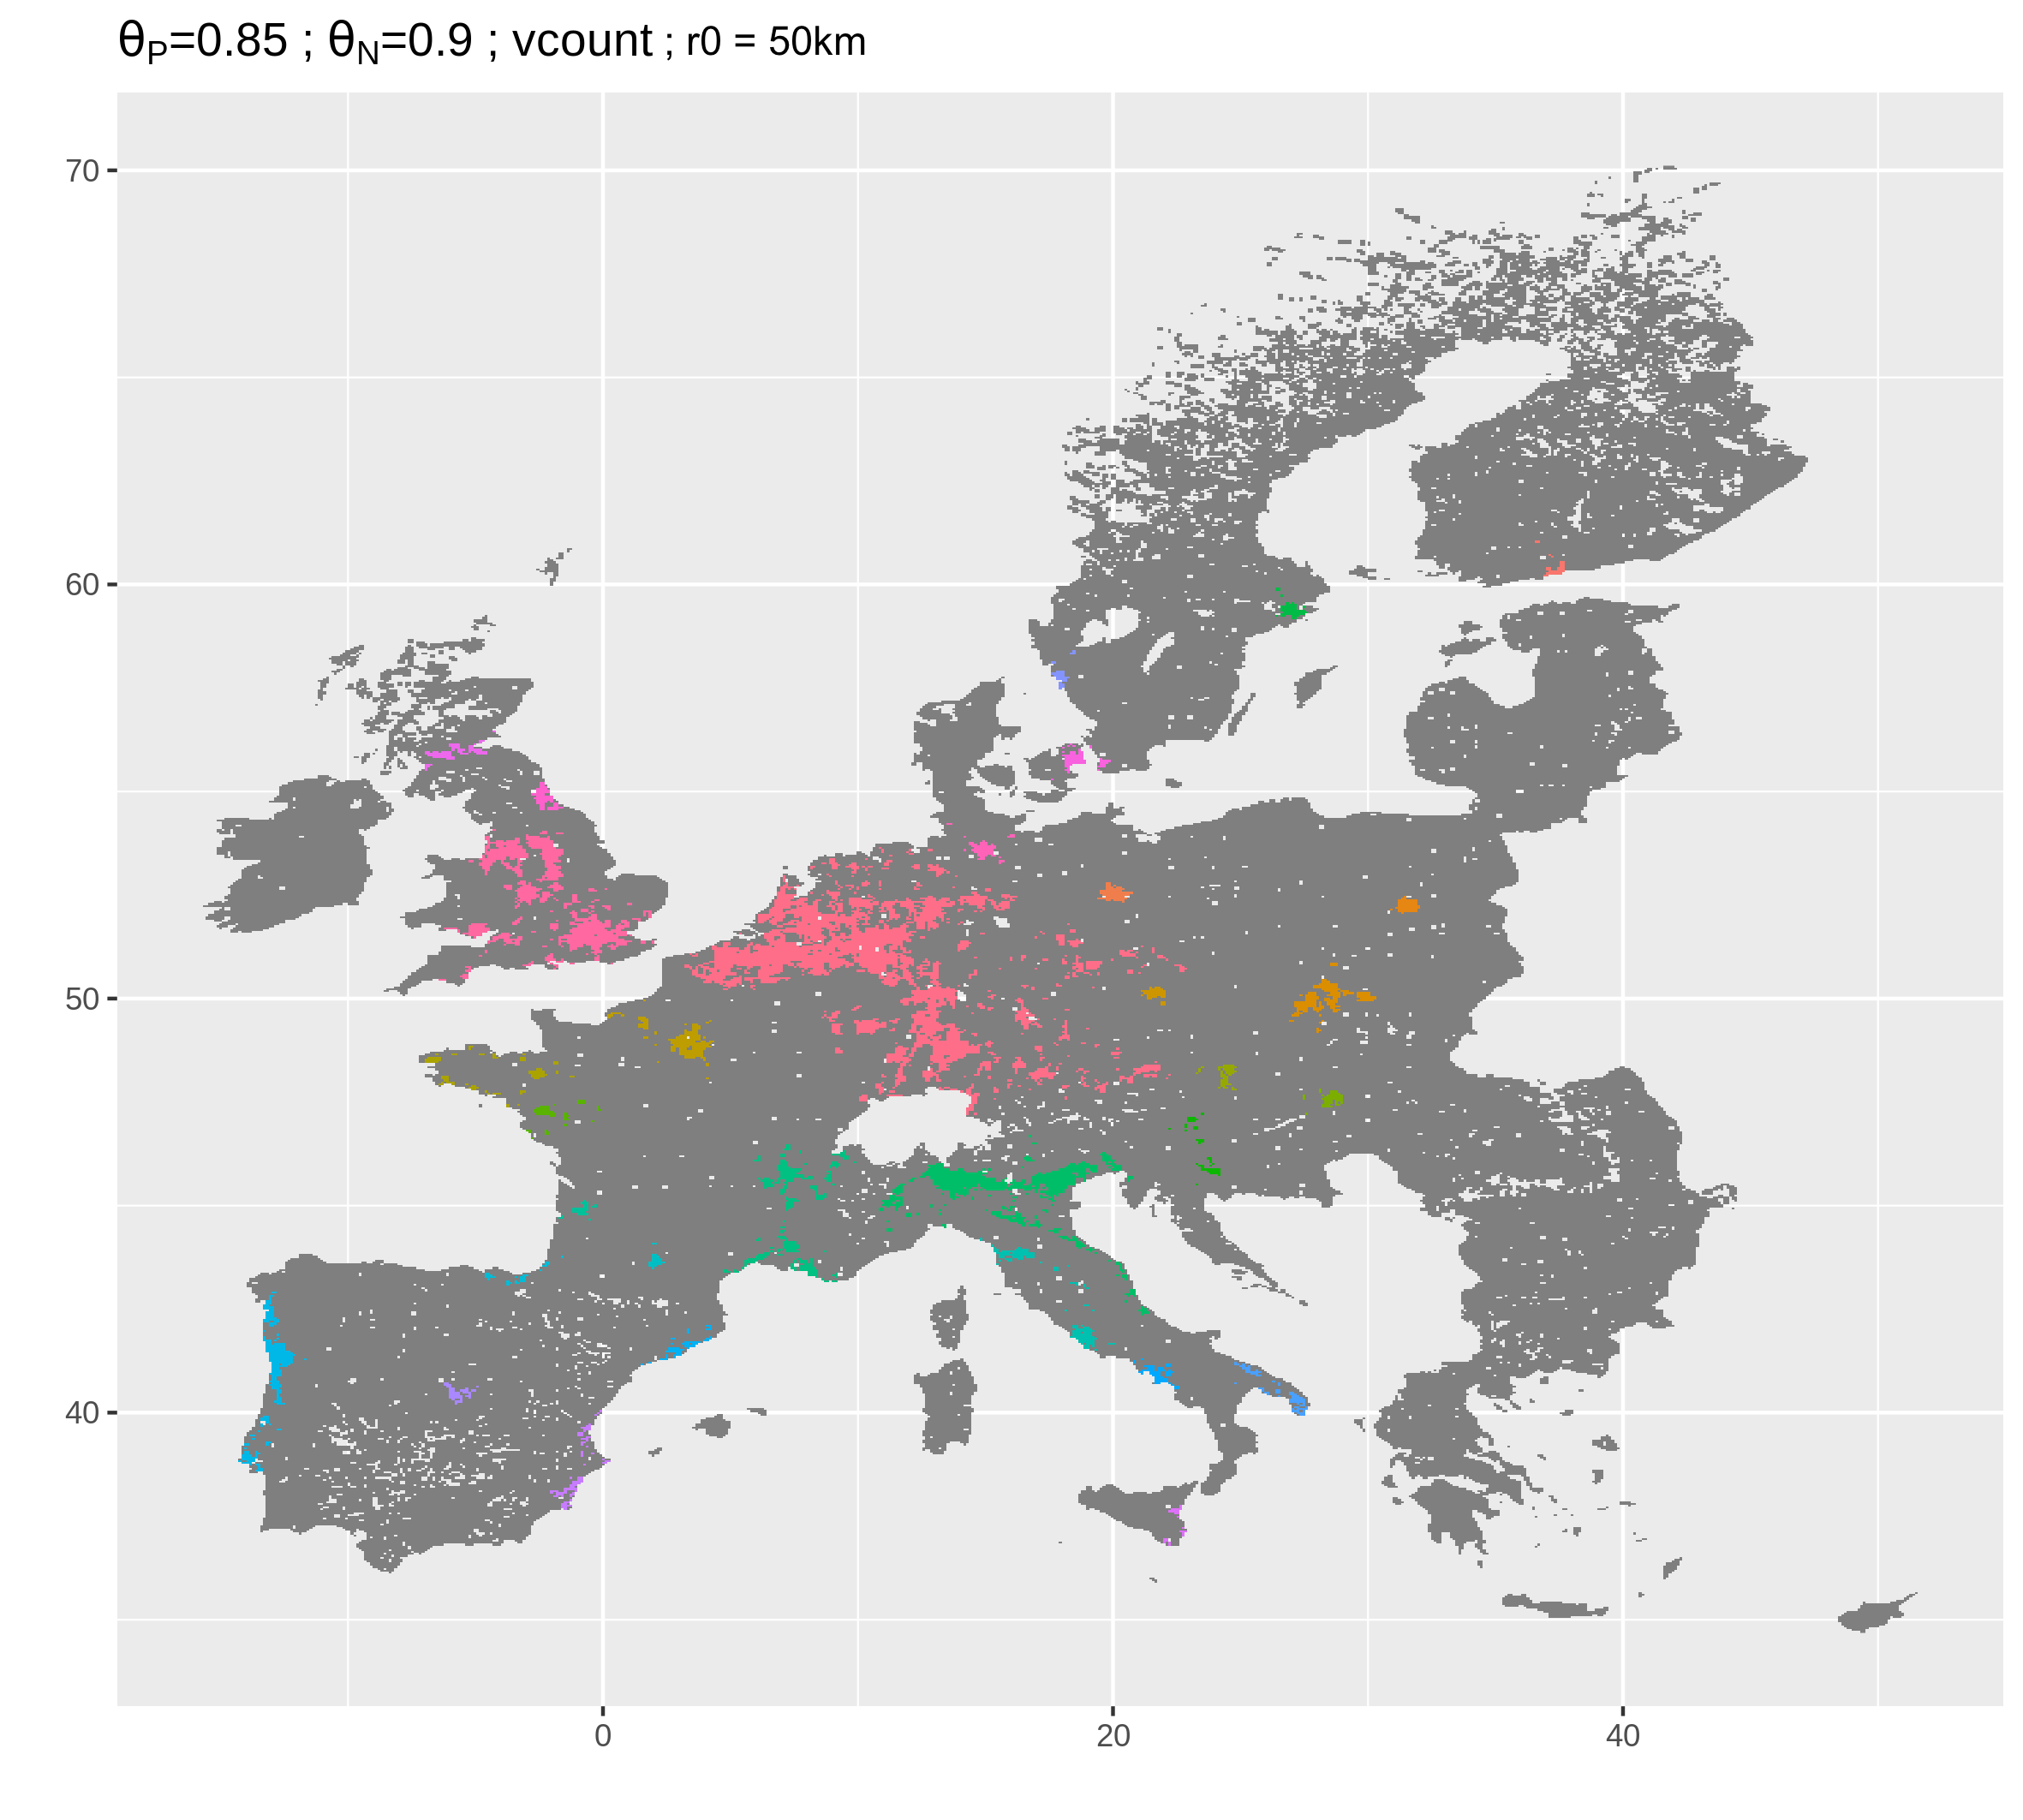
\includegraphics[width=0.49\linewidth]{figures/totalPop1474347_36891685_vcount595_radius50000.png}}
  \centering
  \label{fig:exclusters}
  \caption{Two examples of obtained clusters for different parameter values.}
\end{figure*}
%%%%%%%%%%%%%%%%%%%%





\subsection{Pareto fronts for sustainability}


We show therein that different population, network and distance thresholds yield different performances in terms of sustainability, exhibiting a Pareto front. This suggests policies in terms of regional integration to increase the sustainability of mega-city regions.

%\textit{Superposing Pareto front for observed population and emissions, on all clusters.}
%\includegraphics[height=0.8\textheight]{figures/}

%%%%%%%%%%%%%%%%%%%%
\begin{figure*}[ht] 
%\resizebox{10cm}{7cm}
  {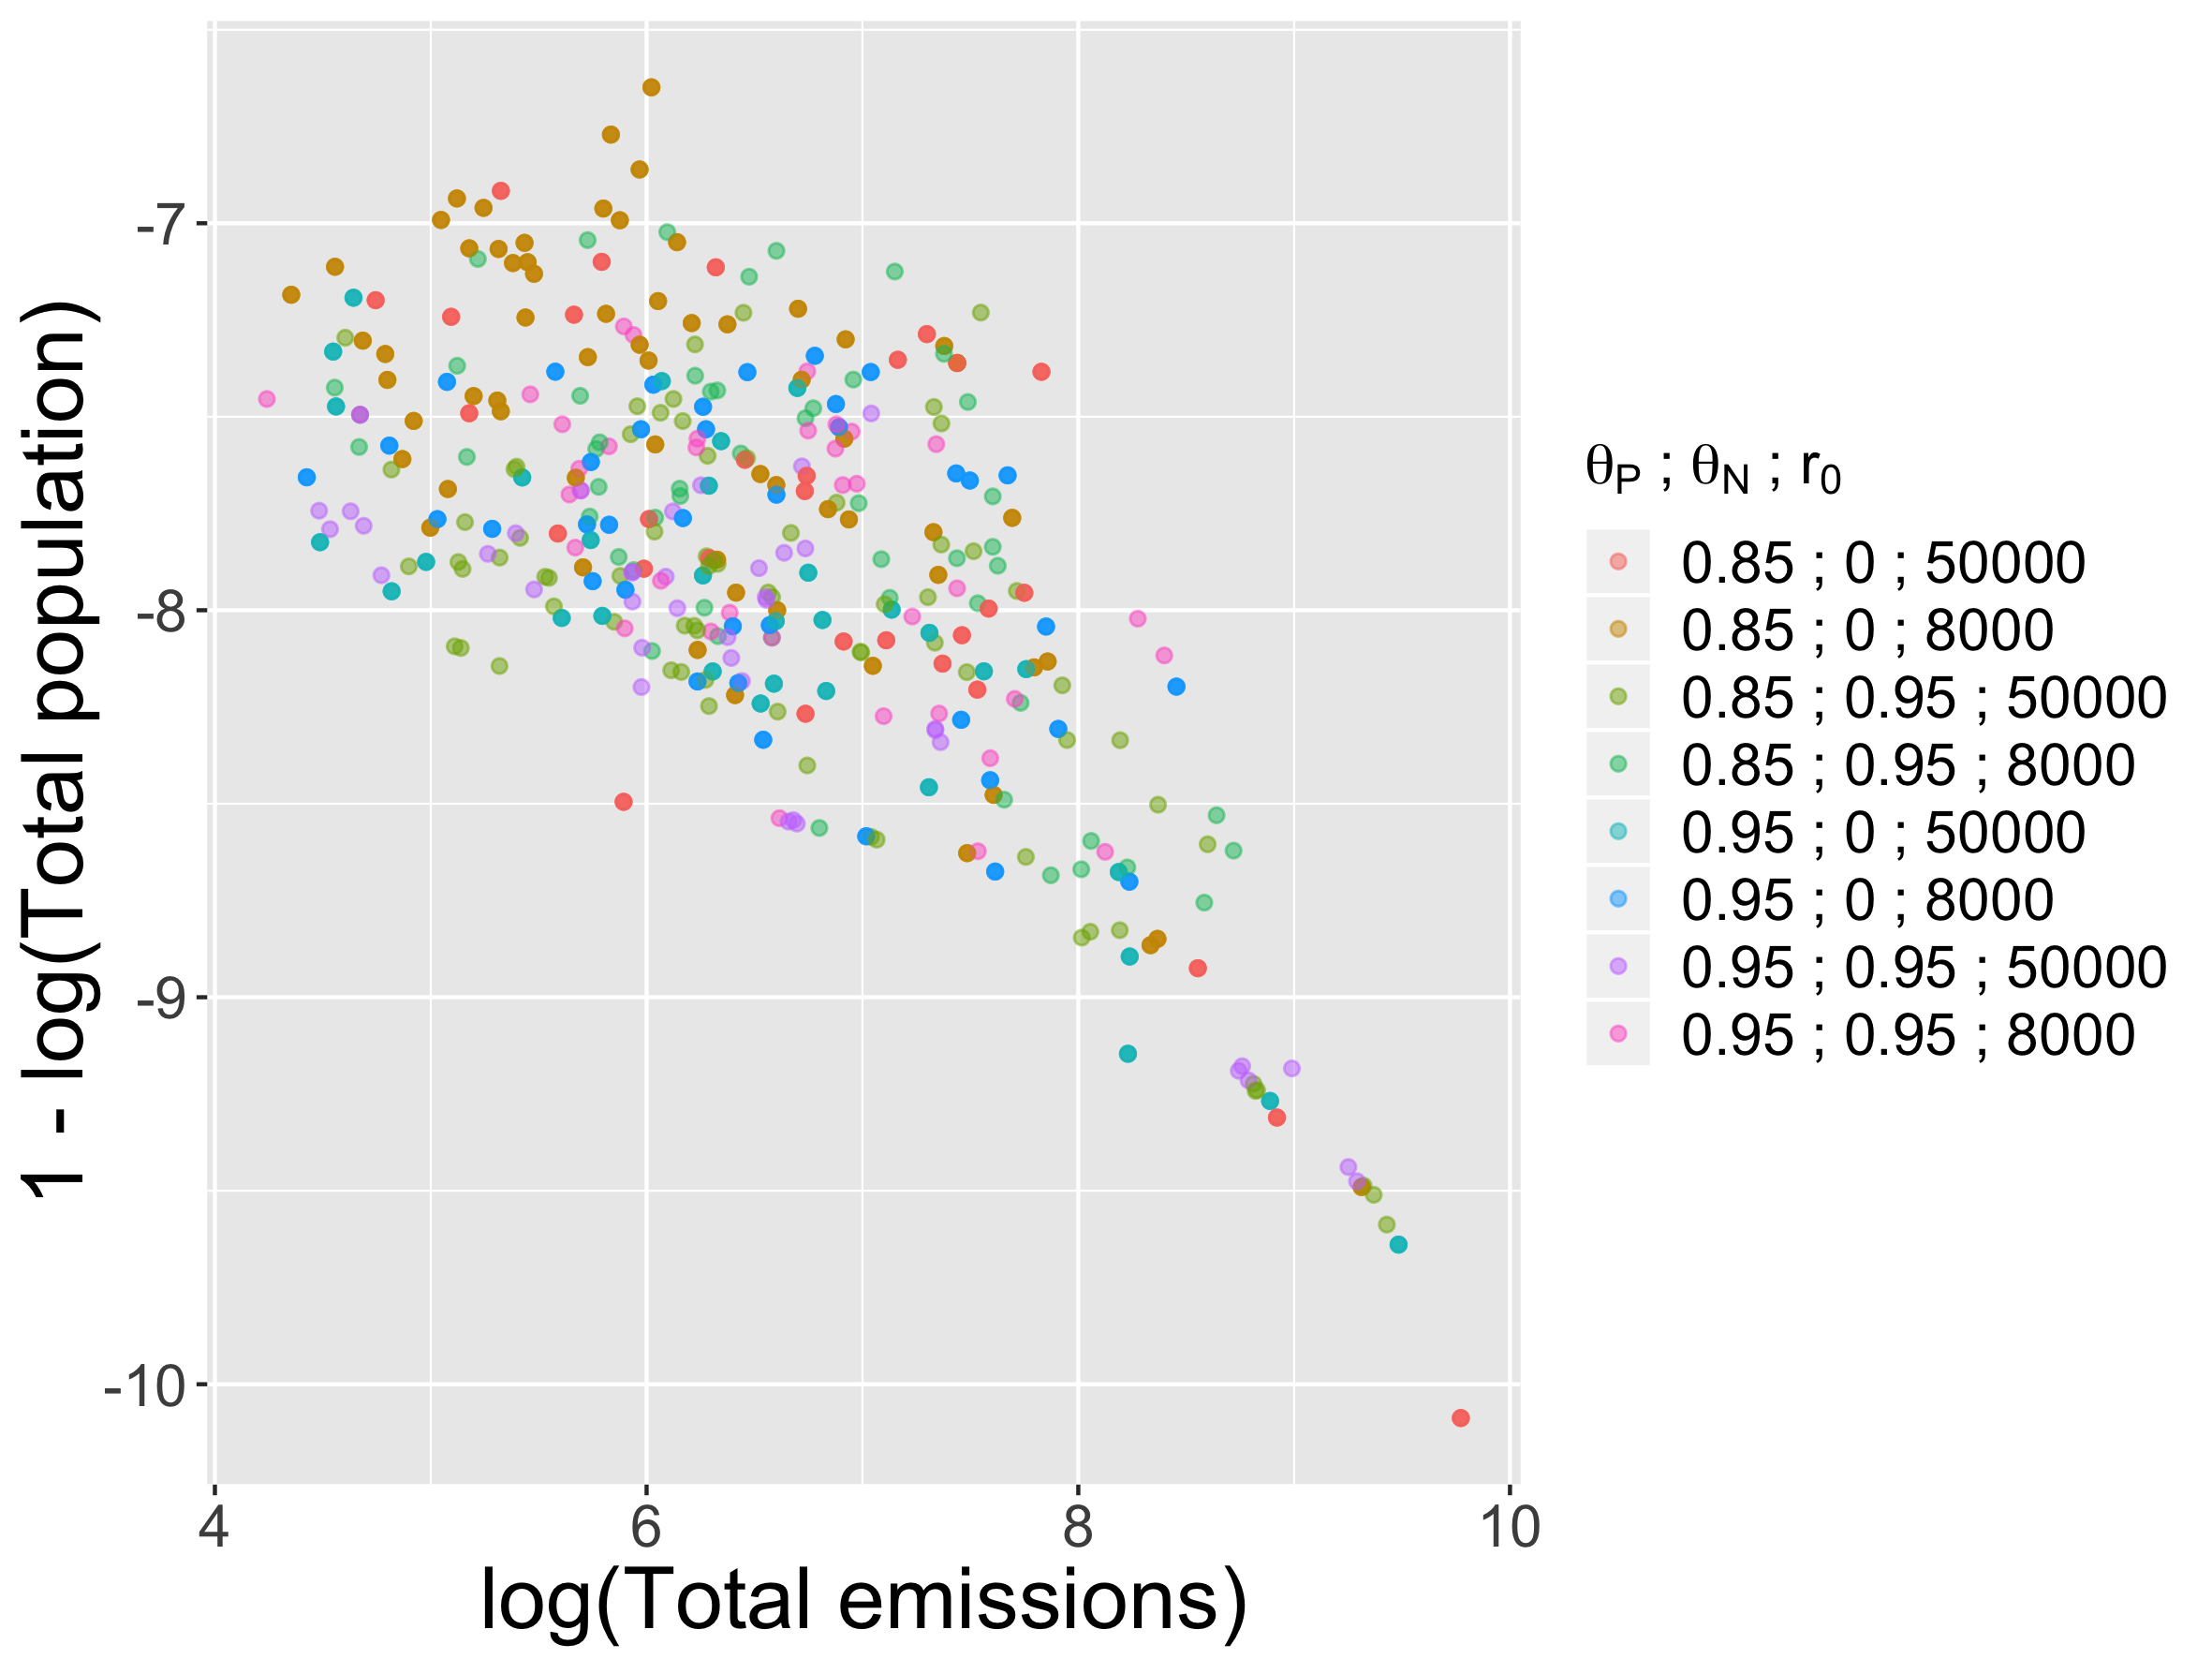
\includegraphics[width=\linewidth]{figures/full_effective_pareto.png}}
  \centering
  \label{fig:paretos}
  \caption{Point clouds of region-level indicators, namely population and emissions, for different parametrizations.}
\end{figure*}
%%%%%%%%%%%%%%%%%%%%


% -> full fronts in reserve slide


% Pareto fronts for aggregated indicators}{
%\textit{Aggregated sustainability indicators suggest some configurations are more Pareto efficient (high $\gamma$ regime, activities with high added value).}

%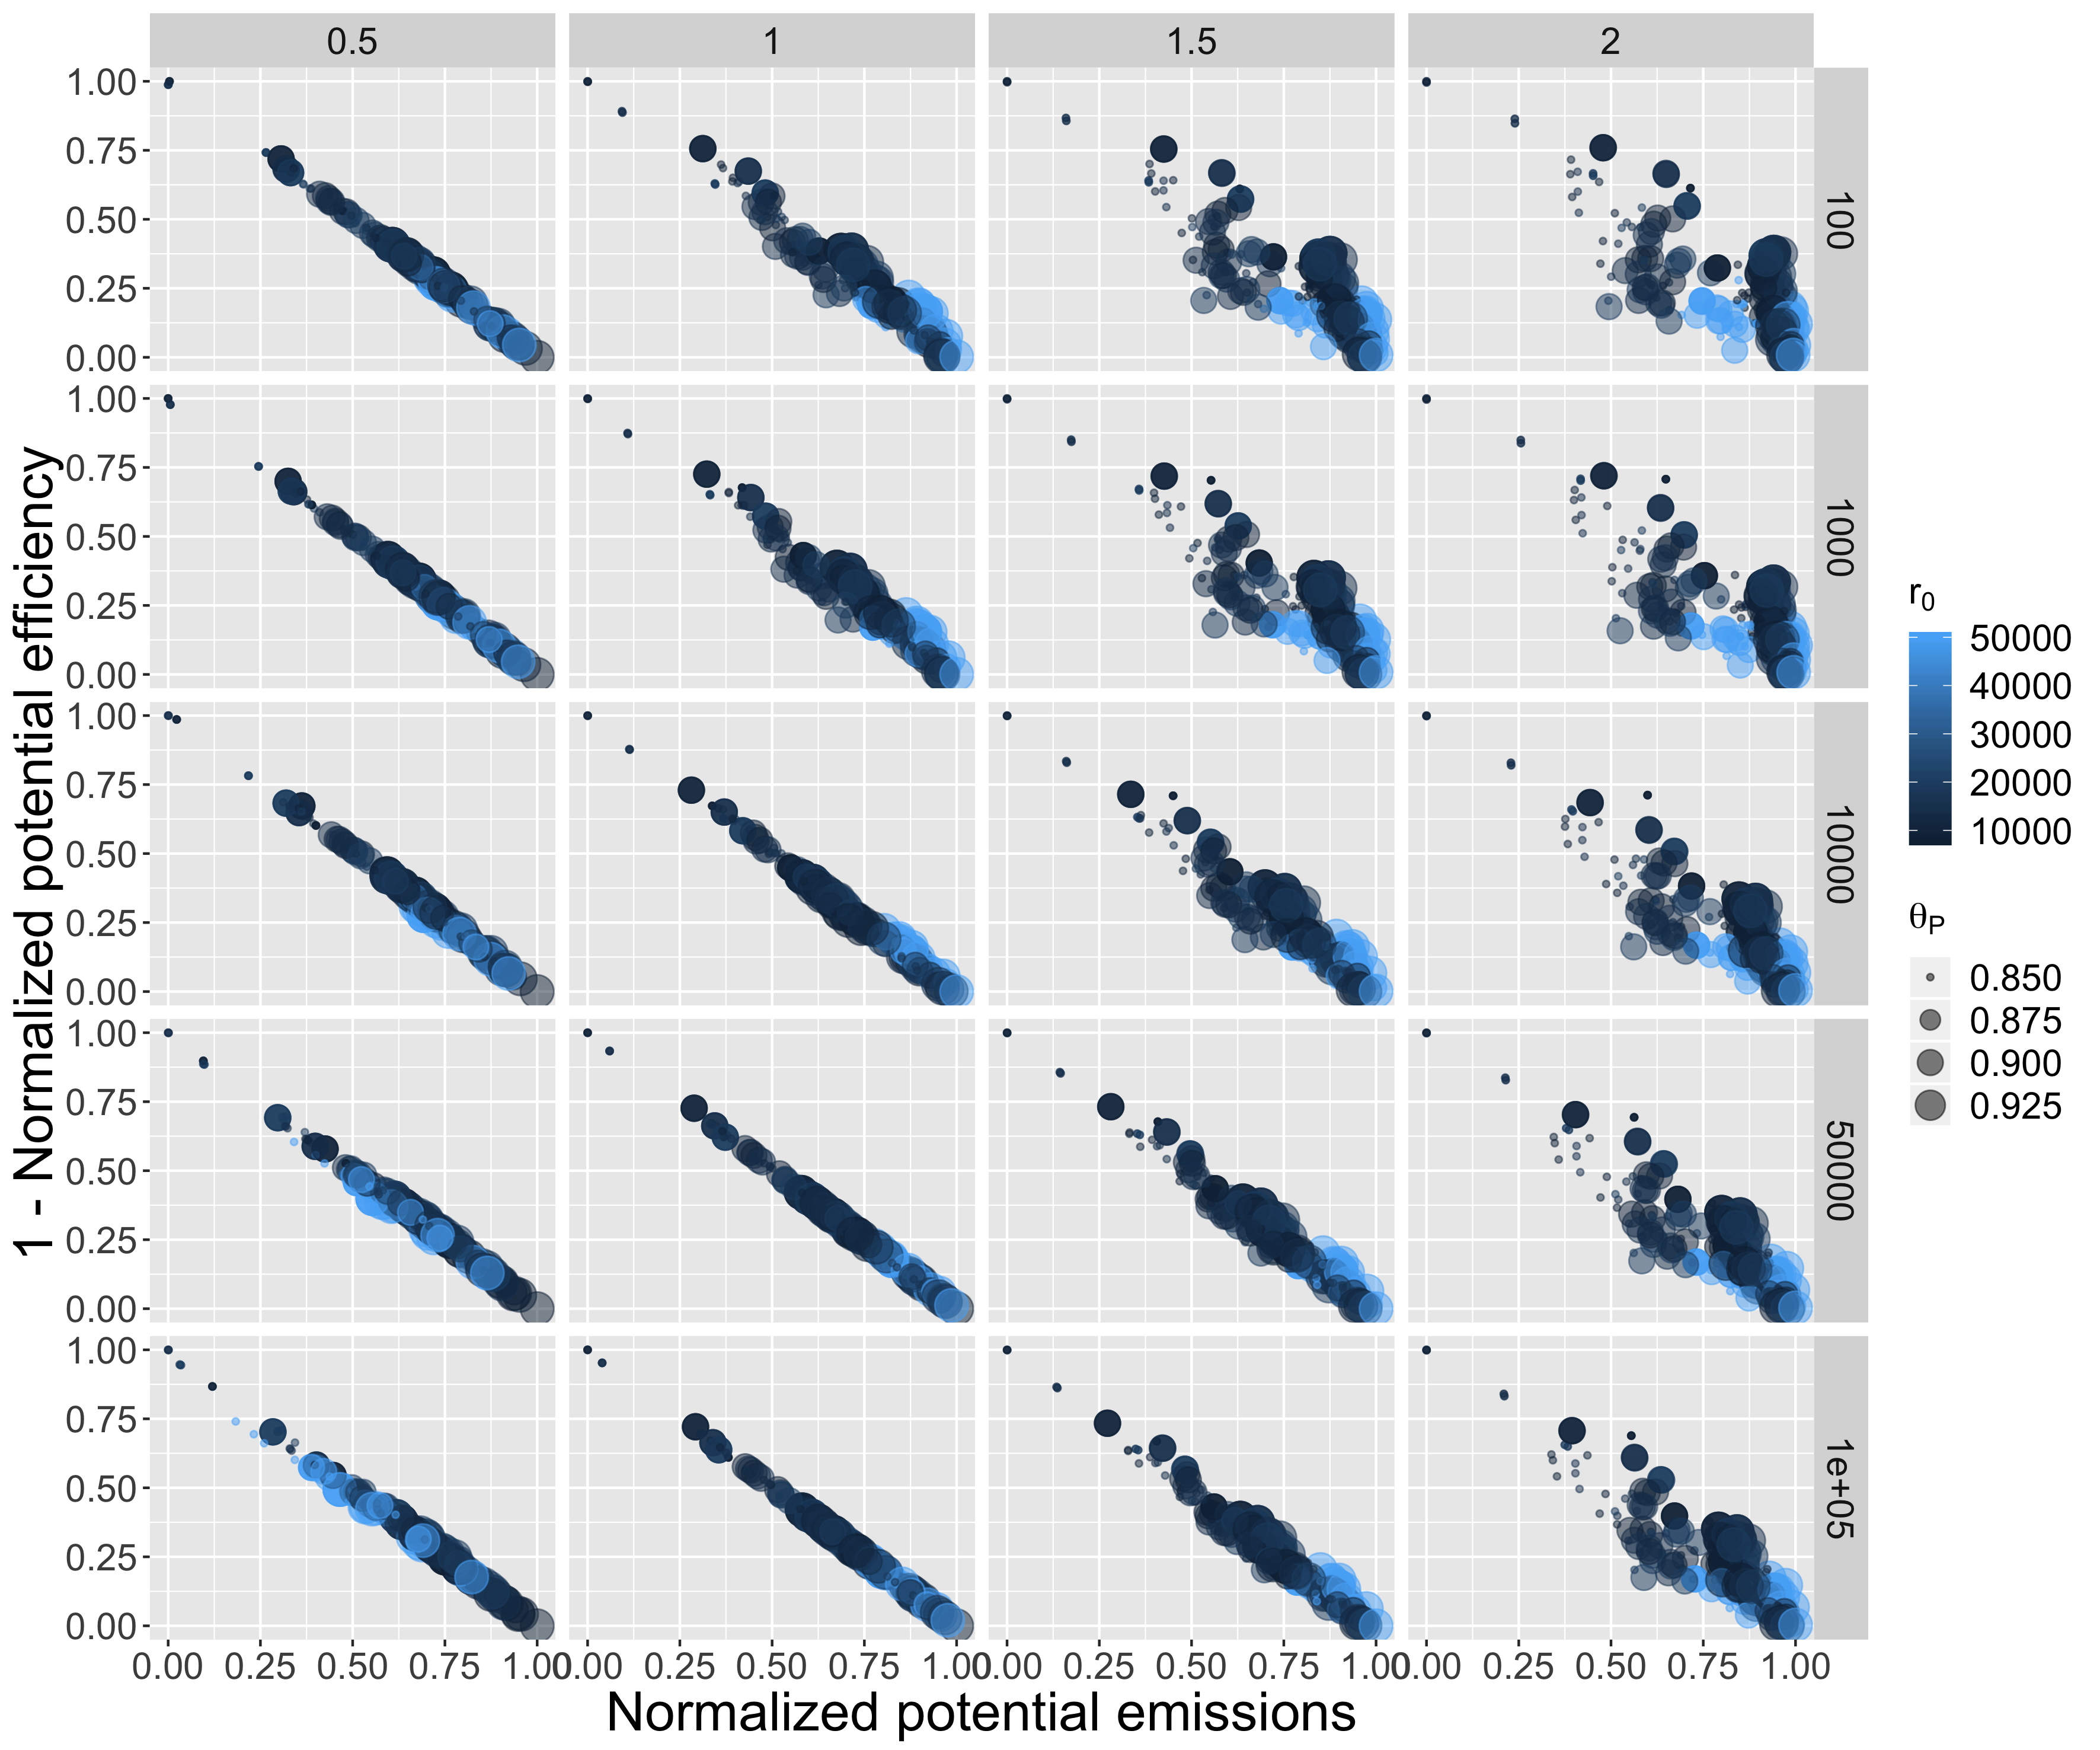
\includegraphics[height=0.8\textheight]{figures/aggreg_paretos_radiuspopthq.png}





%%%%%%%%%%%%%
\subsection{Linking urban morphology and sustainability}


%# Cumulative Proportion  0.7296 0.9650 0.99761 1.00000
%                PC1       PC2         PC3         PC4
%moran   -0.3088585 0.9493848 -0.04444327  0.03605266
%avgdist  0.5417362 0.1415668 -0.82239570 -0.10072759
%entropy  0.5108424 0.2140447  0.45847647 -0.69499942
%slope    0.5917502 0.1811415  0.33390034  0.71100630

When considering the aggregated indicators for a parametrization of endogenous city regions, one can relate them to morphological indicators, computed by~\cite{}, that we average on areas. This establishes a link between urban morphology and sustainibility. A principal component analysis on considered points yield 96\% of variance with two components, and 73\% explained by the first component alone. The first component relates to a level of monocentricity ($PC1 = -0.3\cdot I + 0.54 \cdot \bar{d} + 0.51\cdot \varepsilon + 0.59 \cdot \alpha$). As shown in Fig.~\ref{fig:emissions-pc1}, there seems to exist an optimal intermediate level of monocentricity regarding emissions only, except for long-range and low-hierarchy interactions. However, when considering both emissions and economic indicators, urban form then acts as a compromise variable, moving points on Pareto fronts, as shown in Fig.~\ref{fig:paretos-relative}. In some case, highly monocentric areas can be a good compromise, whereas the intermediate optimal for emissions may yield highly inefficient areas.



%%%%%%%%%%%%%%%%%%%%
\begin{figure*}[ht] 
%\resizebox{10cm}{7cm}
  {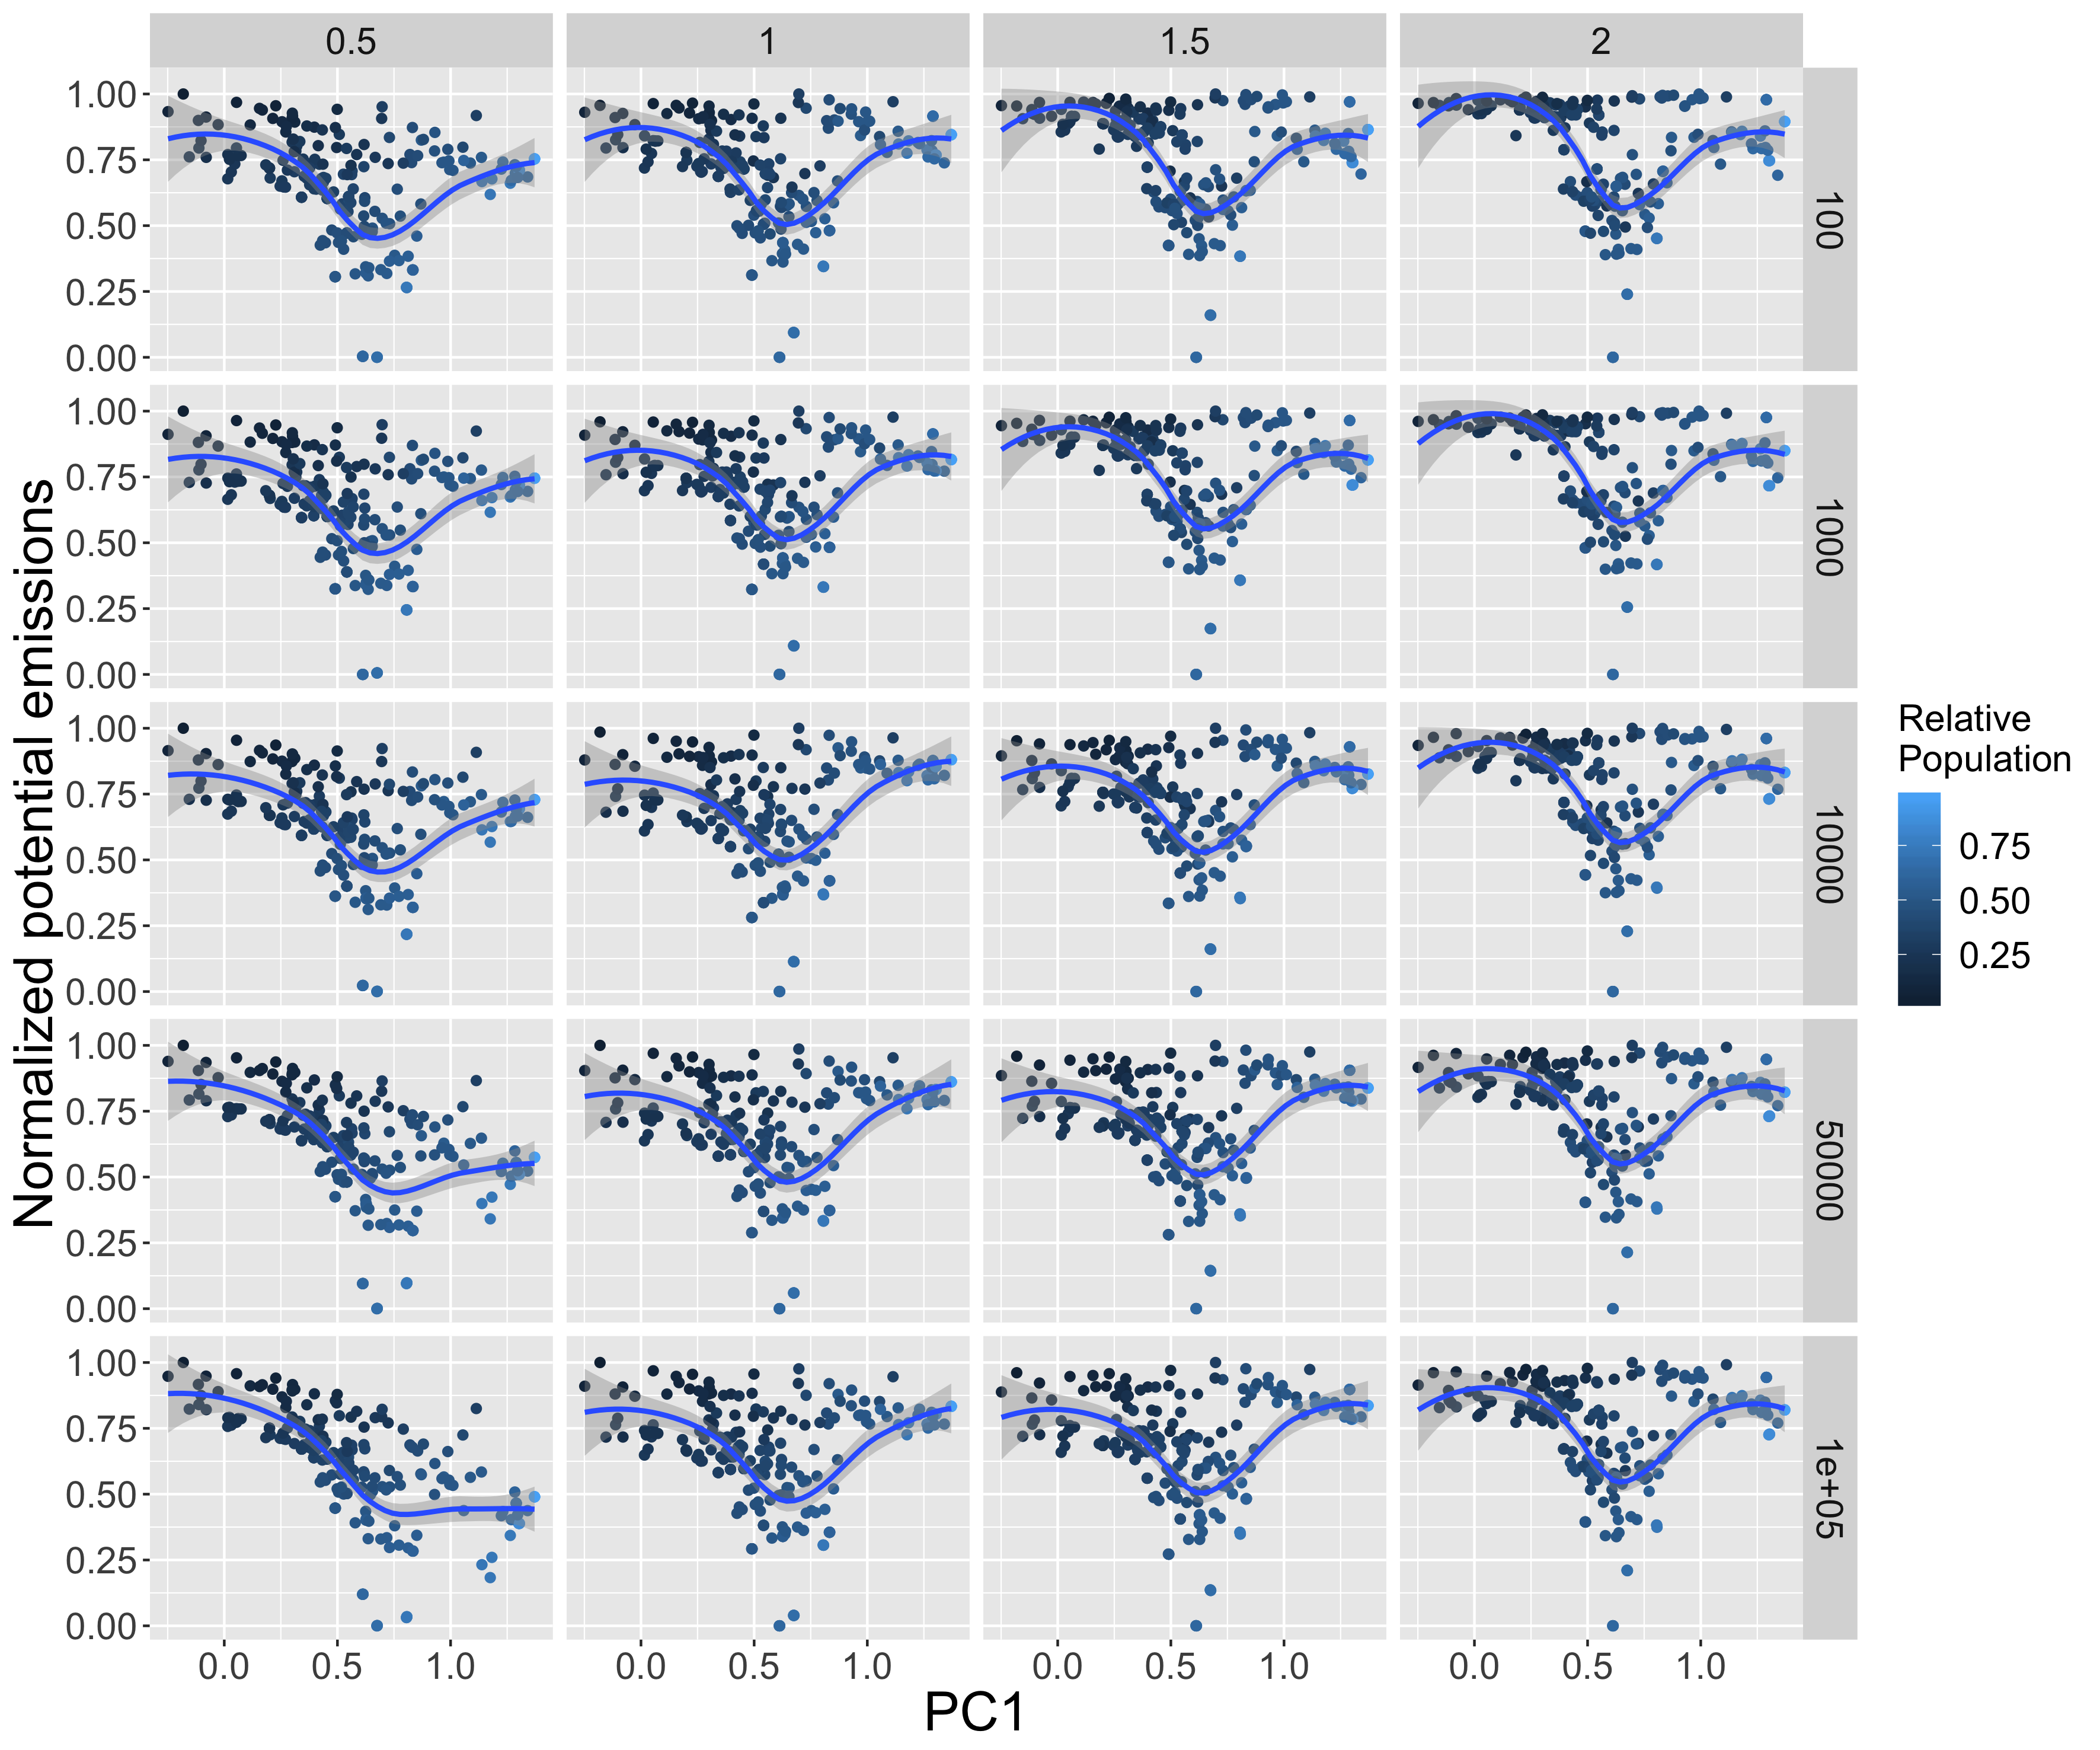
\includegraphics[width=\linewidth]{figures/aggreg_morpho_pc1-emissions.png}}
  \centering
  \label{fig:emissions-pc1}
  \caption{Aggregated values of normalized potential emissions, as a function of the first morphological principal component (PC1), for varying values of parameters $d_G$ and $\gamma_G$. As PC1 is mainly linked to monocentricity, there seems to exist an optimal intermediate level of monocentricity for emissions alone.}
\end{figure*}
%%%%%%%%%%%%%%%%%%%%





%Morphological trade-offs


%\textit{No ``optimal'' cities, different forms yield different compromises in terms of relative indicators.}

%%%%%%%%%%%%%%%%%%%%
\begin{figure*}[ht] 
%\resizebox{10cm}{7cm}
  {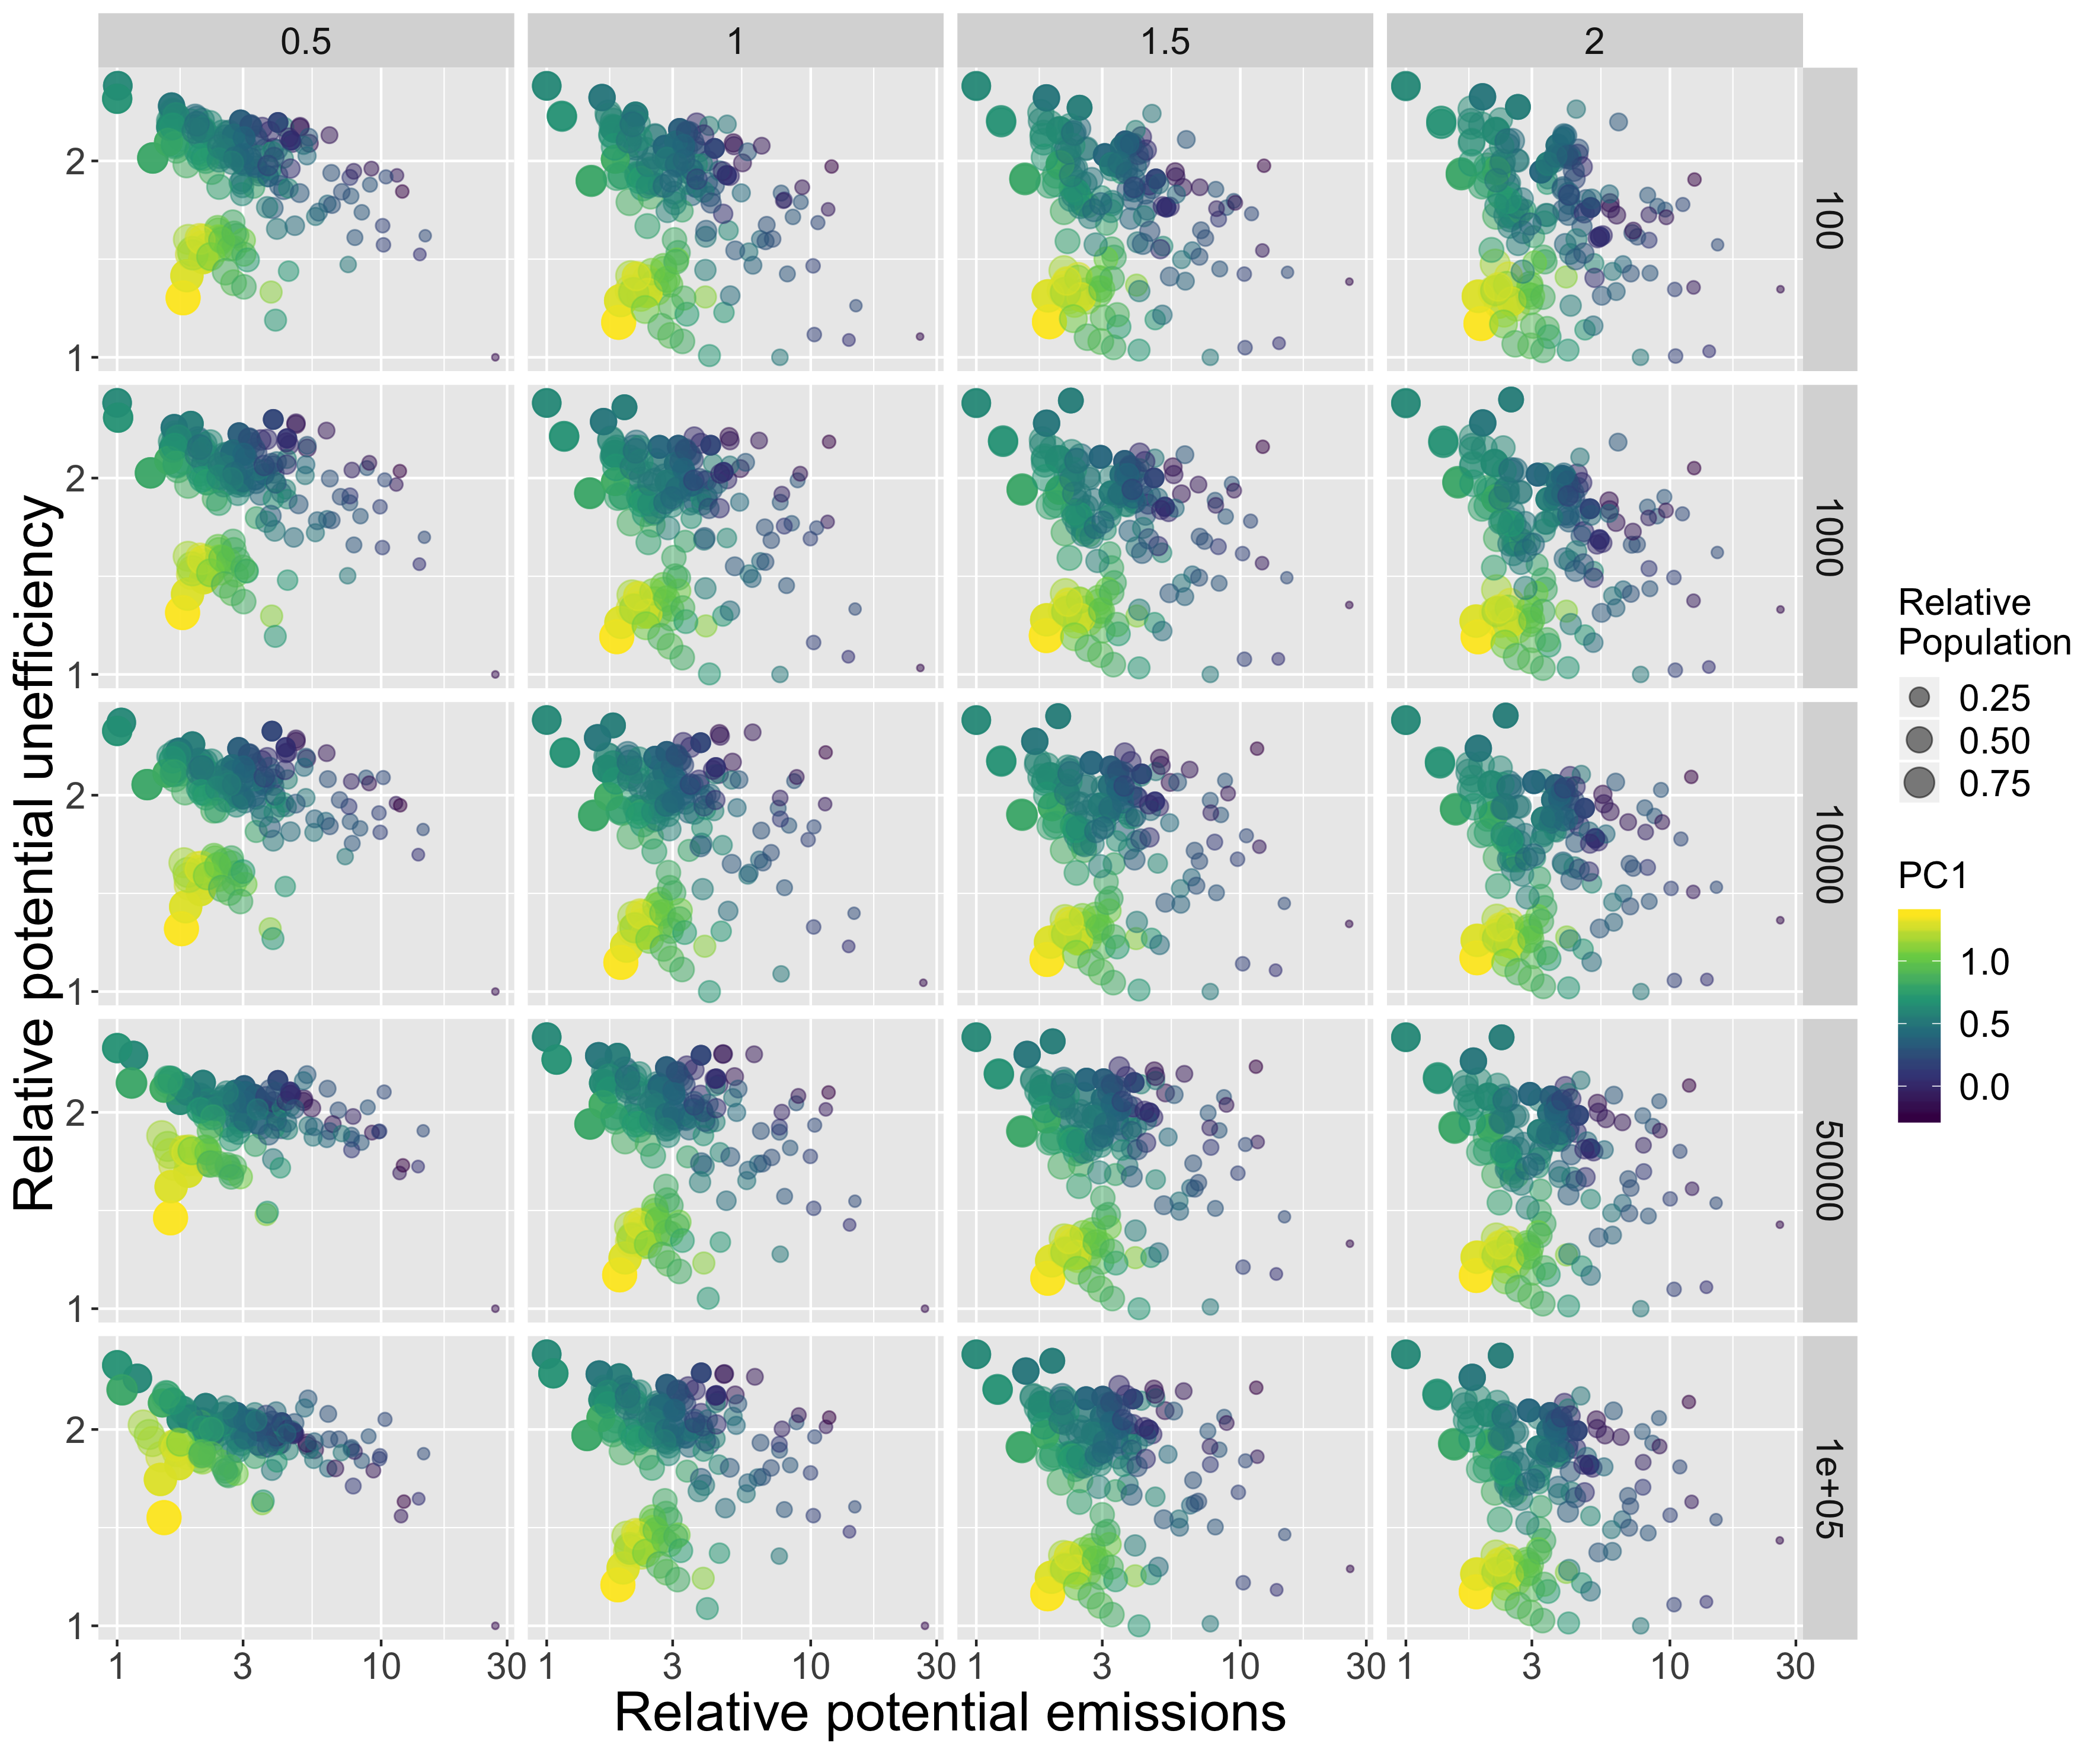
\includegraphics[width=\linewidth]{figures/aggreg_morpho_relemissions-relefficiency_colpc1_logscale.png}}
  \centering
  \label{fig:paretos-relative}
  \caption{Relative potential emissions against relative potential economic unefficiency (both indicators should be minimized), for varying values of $\gamma_G$ (columns) and $d_G$ (rows). Color level gives the value of PC1, whereas point size gives the share of total population contained within considered areas.}
\end{figure*}
%%%%%%%%%%%%%%%%%%%%







\section{Discussion}

Further work can consist in the use of calibration heuristics \citep{reuillon2013openmole} to find in a more robust way optimal parameter values.


% -> depending on results


%Grid sampling to explore regions rapidly limited

%$\rightarrow$ towards the use of genetic algorithms on grid, made smooth with the OpenMOLE software \url{https://next.openmole.org/}
%
\includegraphics[height=0.35\textheight]{figures/openmole.png}
%\footnotesize \textit{OpenMOLE: (i) embed any model as a black box; (ii) transparent access to main High Performance Computing environments; (iii) model exploration and calibration methods.}
%\textbf{Apply to the summer school !} \url{https://exmodelo.org/}


%\textbf{Implications}

%$\rightarrow$ Multi-dimensionality of urban systems and a link between form and function captured through multilayer percolation.

%$\rightarrow$ Possible transfer to policy-making recommandations: Pareto-optimal configuration can be used for the planning of regional transportation networks, policies for subsidies, etc.



%\textbf{Developments}


% detail method to extrapolate parameters of gravity flows

% interesting result : compare these emission with the synthetic ? (then just a refinment ?) -> yes, better. show new Pareto fronts with this fixed parameters for only emissions, and varying for economic ? 

%$\rightarrow$ Systematic calibration of parameters to unveil more exhaustive Pareto fronts.

The use of calibration algorithms % TODO finish

Extrapolating transportation flows with a spatially explicit gravity and flow model can allow to compare these with actual transportation flows in the emission database, and yield a possible calibration. These extrapolated parameters could then be used within the economic and emissions potentials.

An other potential development would imply crossing our endogenous definitions of urban regions with socio-economic databases, and compute indicators implied in other dimensions of sustainability, for example related to socio-economic inequalities, spatial distribution of accessibilities, activities with different scaling exponents.
% ex : at least different scaling exponent.



\section{Conclusion}


%$\rightarrow$ Empirical and theoretical research directed towards concrete policy-making applications. \textbf{Need for more data-driven approaches.}
%First step towards systematic benchmarks and multi-modeling. \textbf{Need for more systematic model exploration.} % model coupling / benchmarking

%$\rightarrow$ Towards multi-scalar approaches ? \textbf{Need for more integrated models.}
 %Model integration and multi-scalarity ? \textbf{Need for more integrated models.}

%$\rightarrow$ Multidimensionality of urban systems ? \textbf{Need for more interdisciplinarity.}

%\textbf{Related works}


%Raimbault, J. (2018). Calibration of a density-based model of urban morphogenesis. PloS one, 13(9), e0203516.

%Raimbault, J. (2018). An Urban Morphogenesis Model Capturing Interactions between Networks and Territories. \textit{Forthcoming in Mathematics or Urban Morphogenesis.} arXiv:1805.05195.

%Raimbault, J. (2018). Caract{\'e}risation et mod{\'e}lisation de la co-{\'e}volution des r{\'e}seaux de transport et des territoires (Doctoral dissertation, Université Paris 7 Denis Diderot). \url{https://halshs.archives-ouvertes.fr/tel-01857741}
%\textbf{Open repository} at \texttt{https://github.com/JusteRaimbault/UrbanMorphology} (code, data and results)%\\\smallskip
% no grid used
%\textbf{Acknowledgments}: thanks to the \textit{EGI} for access to the infrastructure.







\bibliographystyle{jimis-en}
\bibliography{biblio}

\appendix\footnotesize

\section{Appendix 1: supplementary sensitivity analyses}



%\sframe{Results: effective emissions}{

%\textit{Effective emissions exhibit a supralinear scaling of population}
%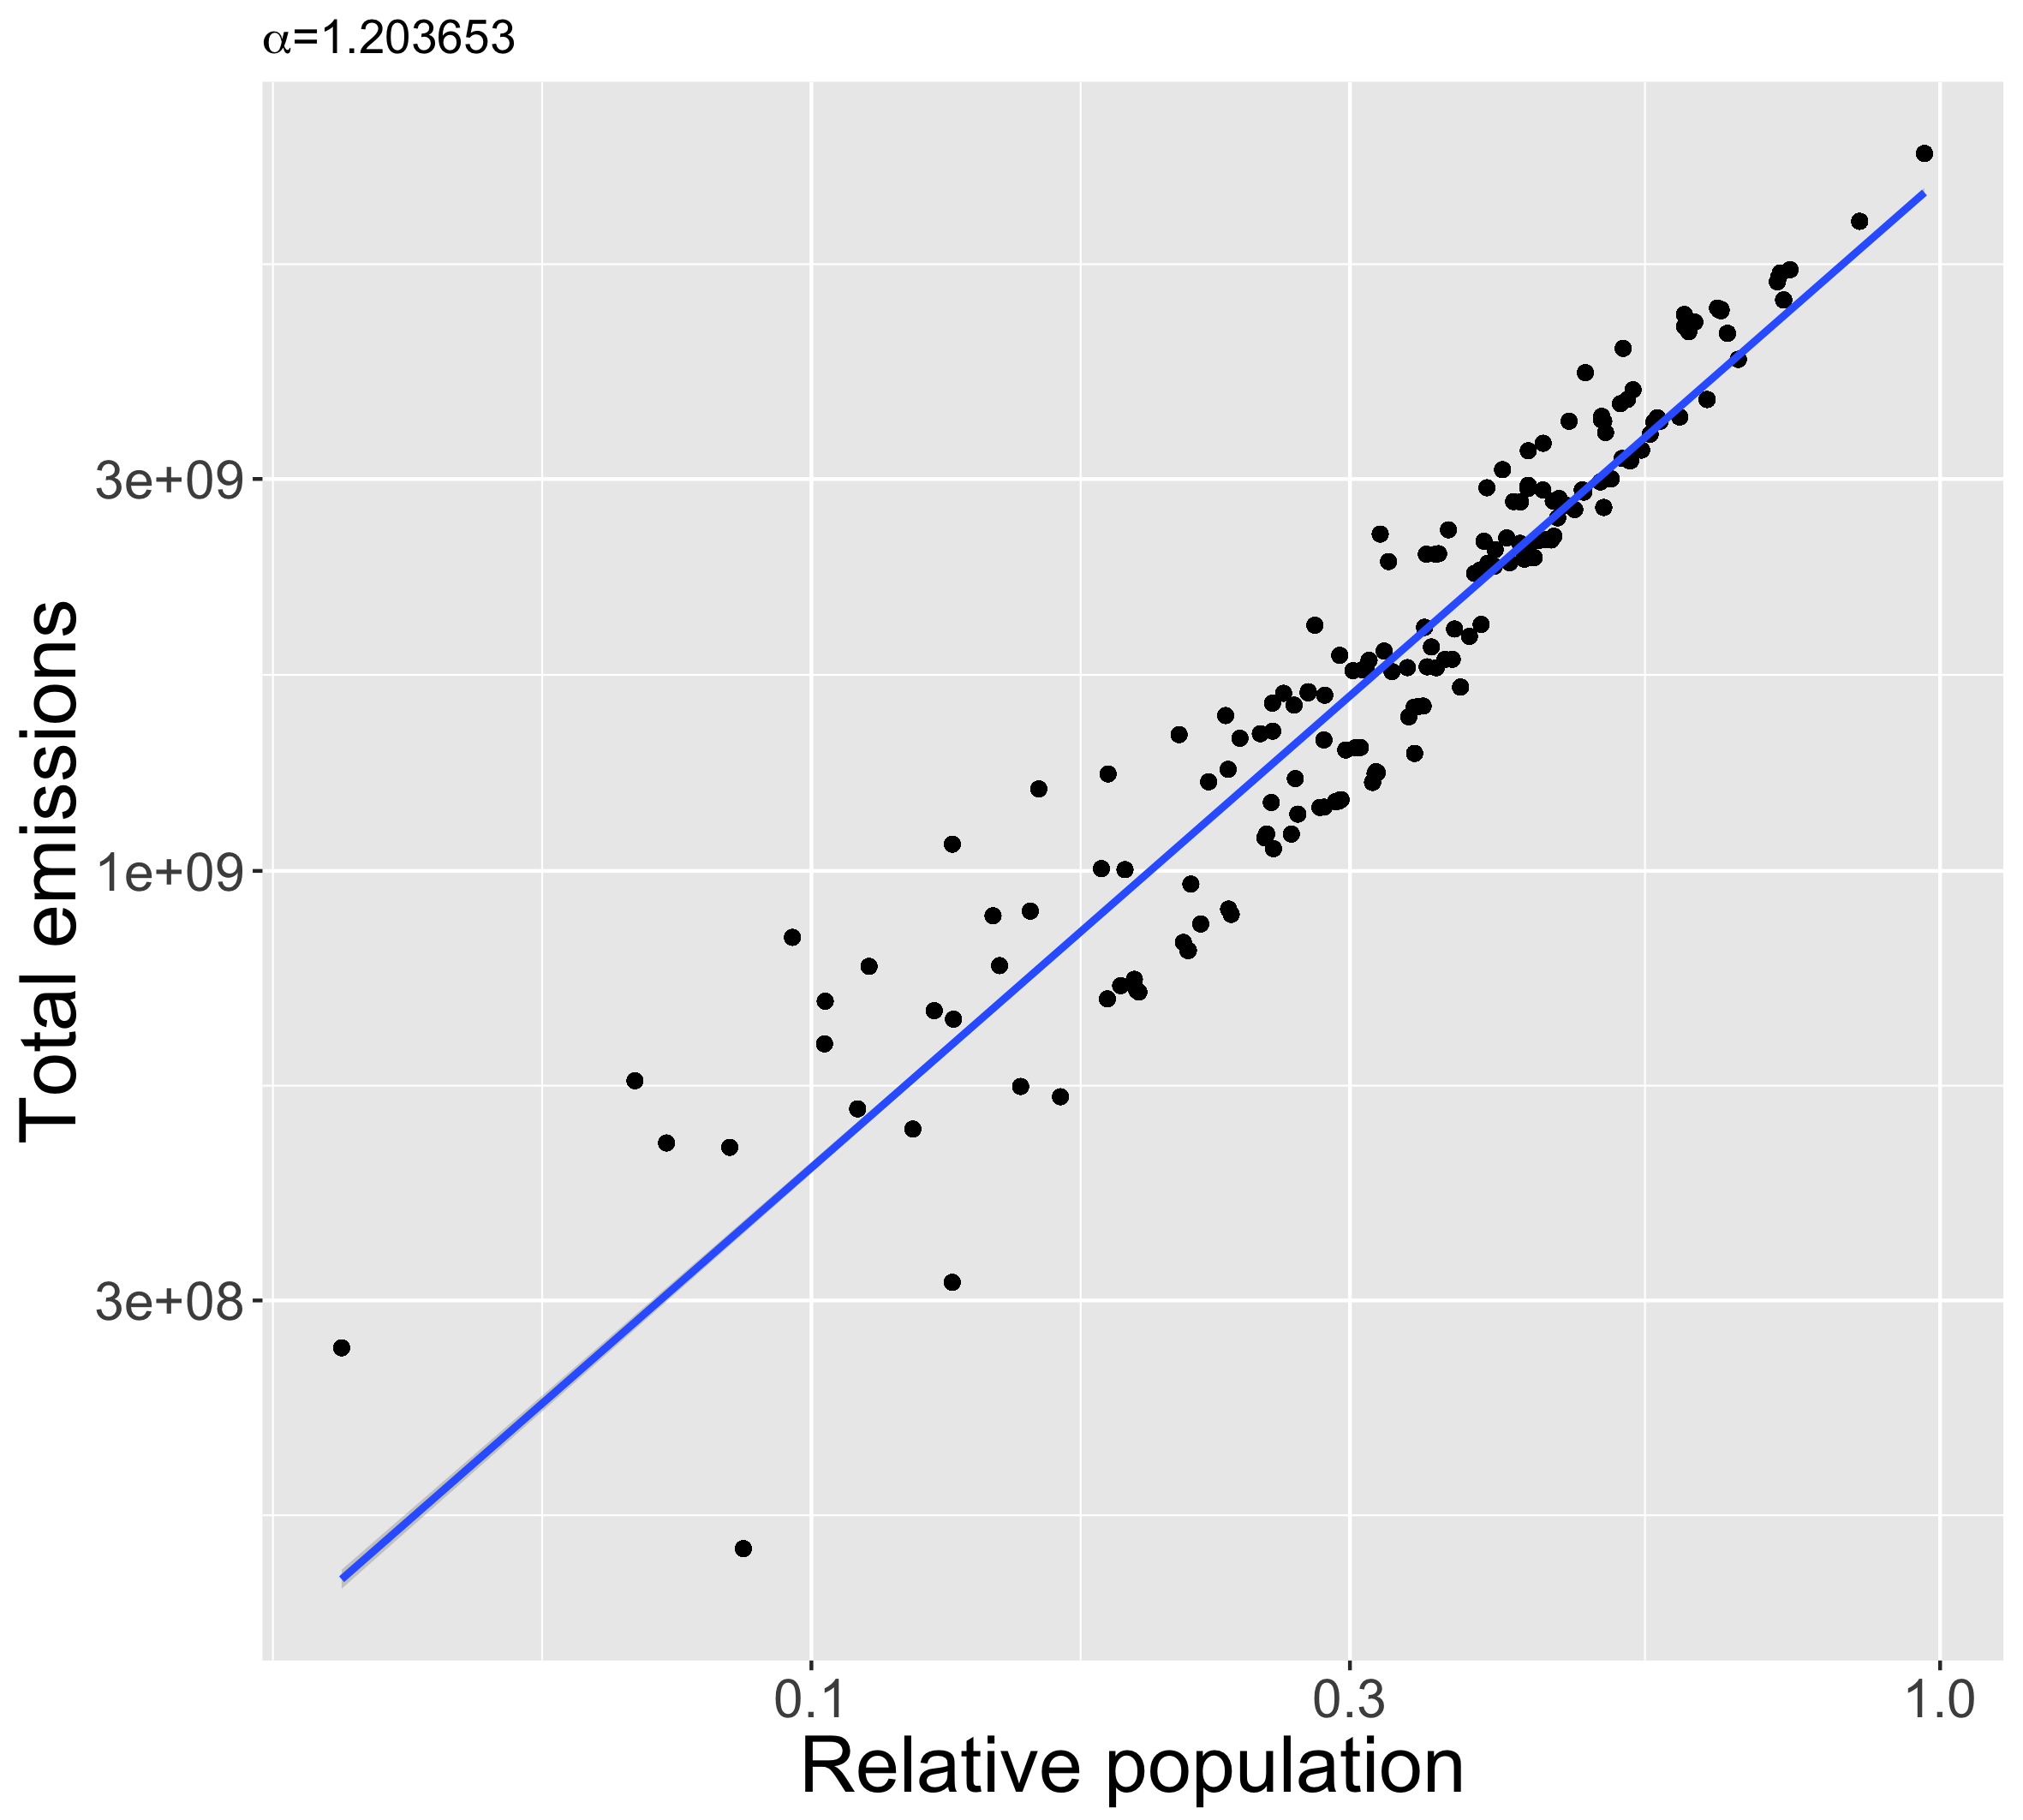
\includegraphics[height=0.83\textheight]{figures/aggreg_effective.png}

%\sframe{Results: all clusters Pareto fronts}{

%\textit{Variation of Pareto front patterns when potential parameter $\gamma,d_0$ vary.}

%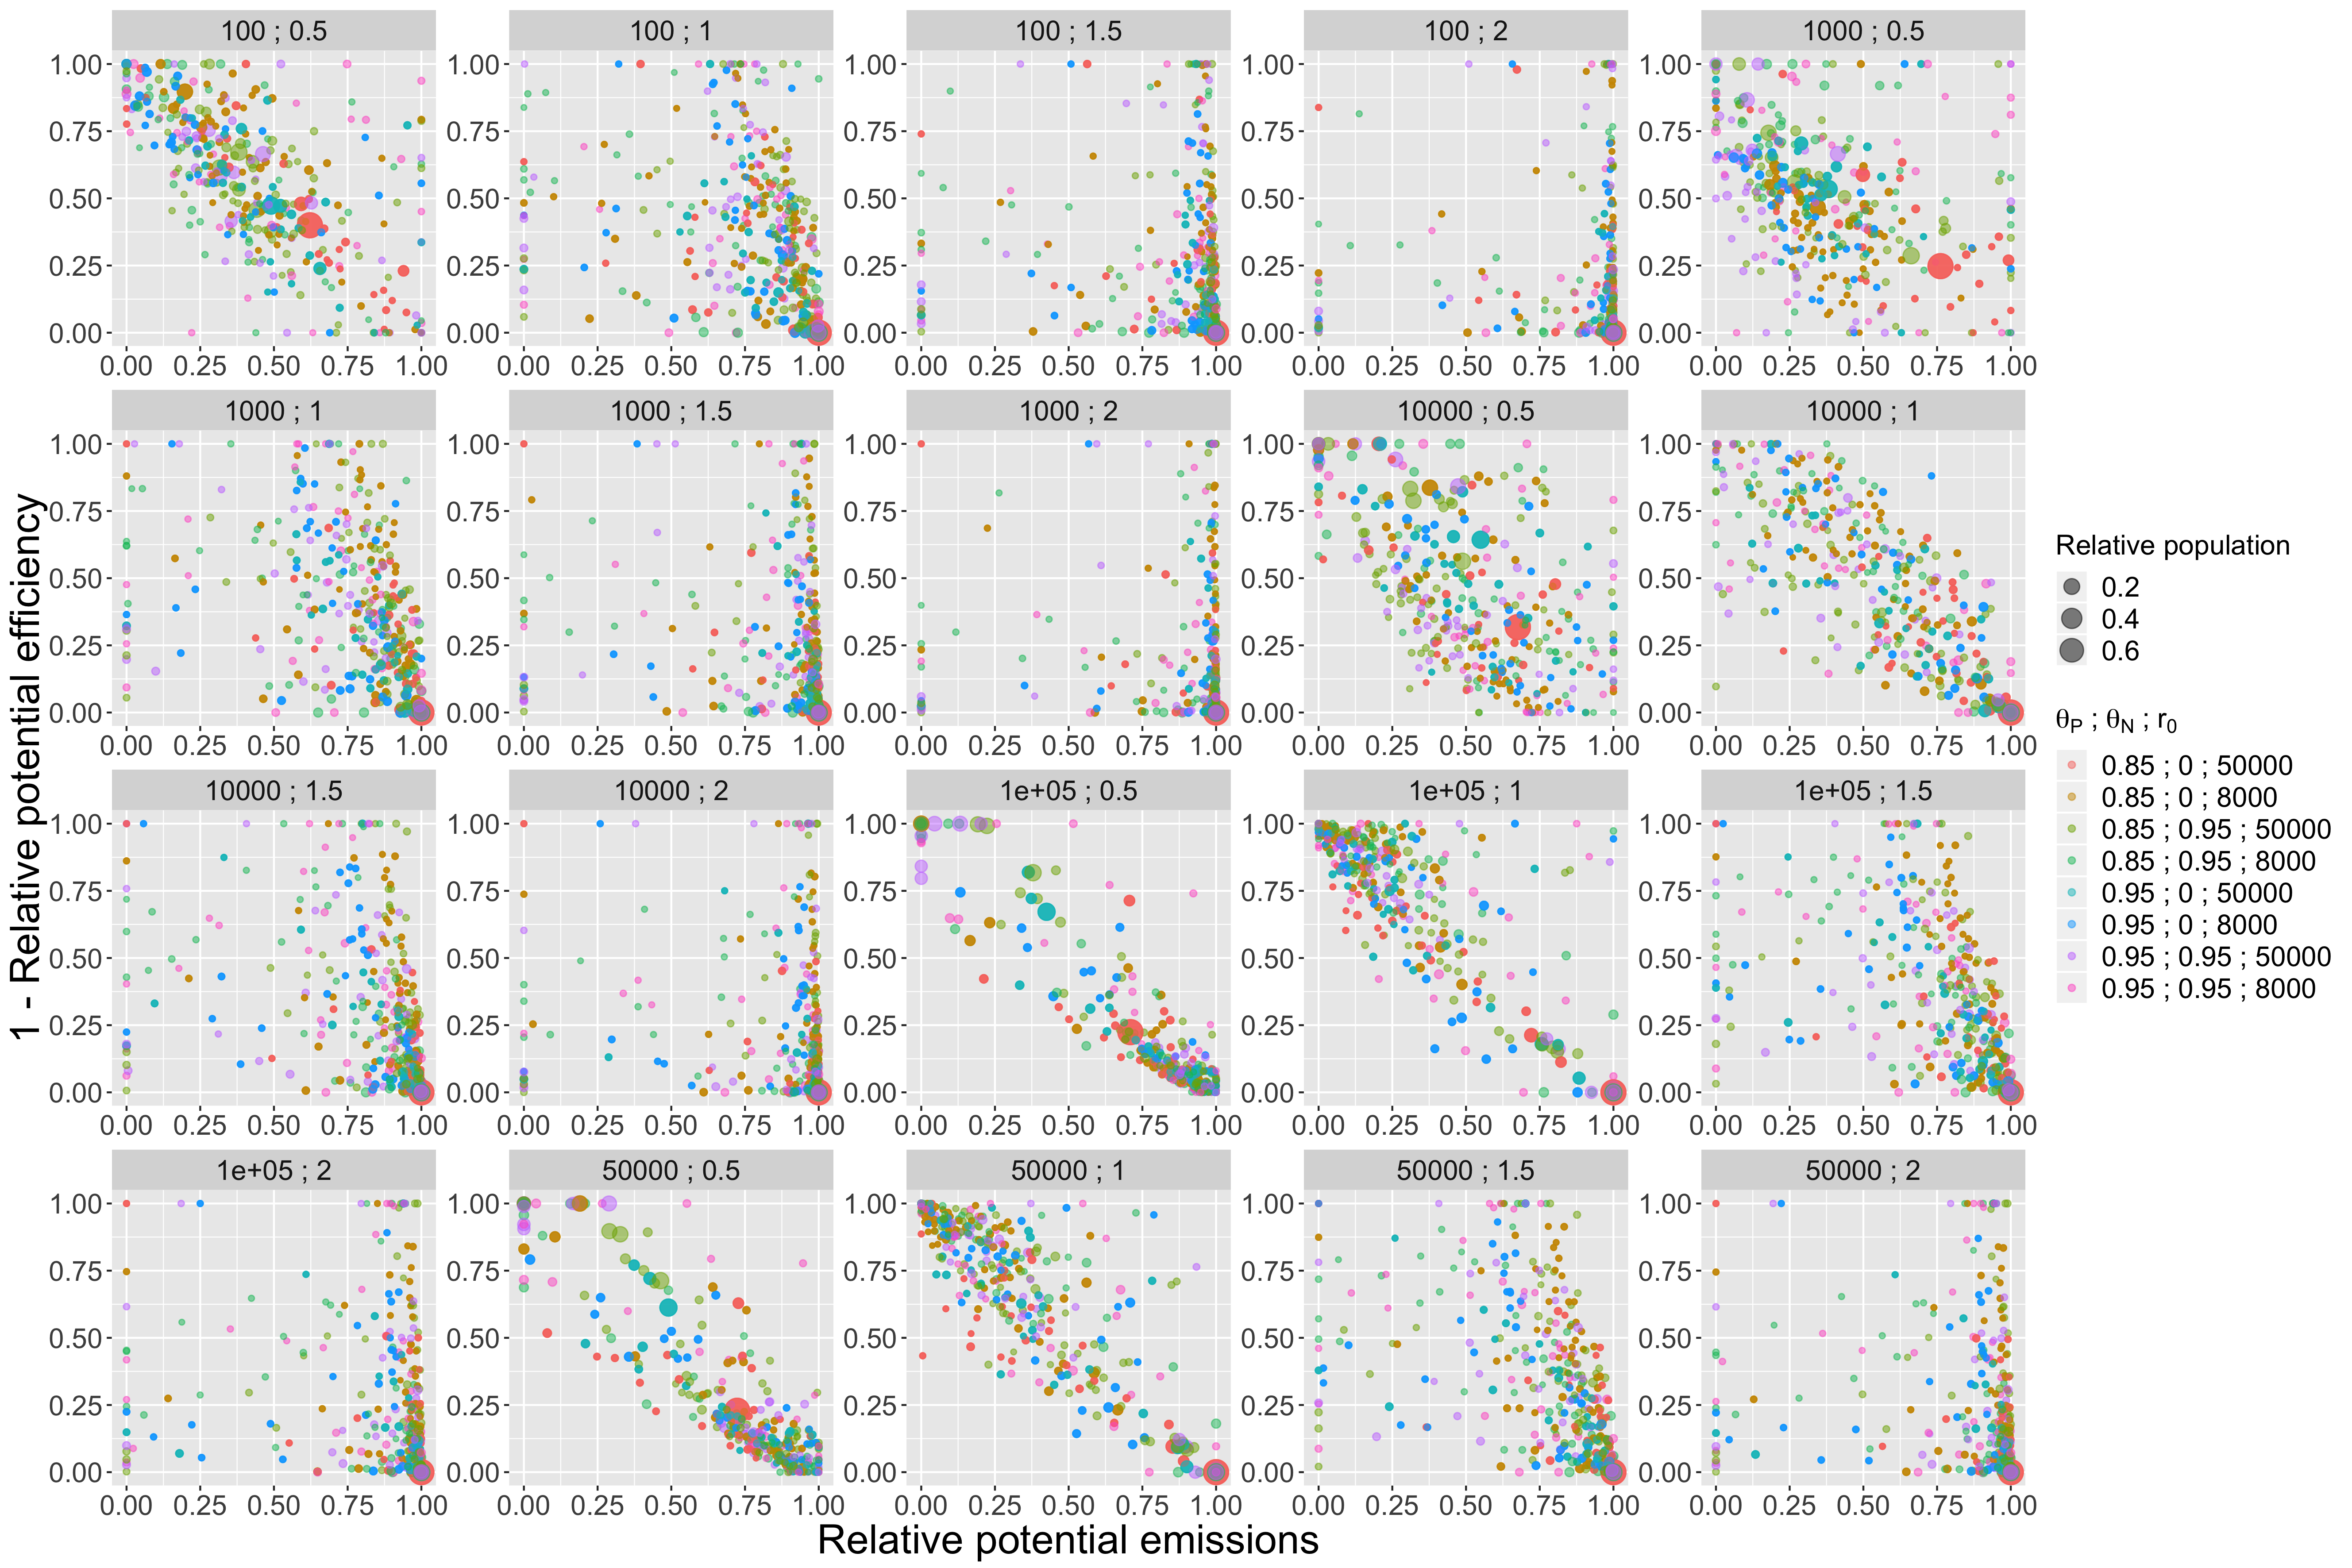
\includegraphics[width=0.9\textwidth]{figures/full_paretos.png}


%\sframe{Results: an optimal morphology}{

%\textit{More monocentric areas are more optimal in terms of relative emissions and efficiency ?}

%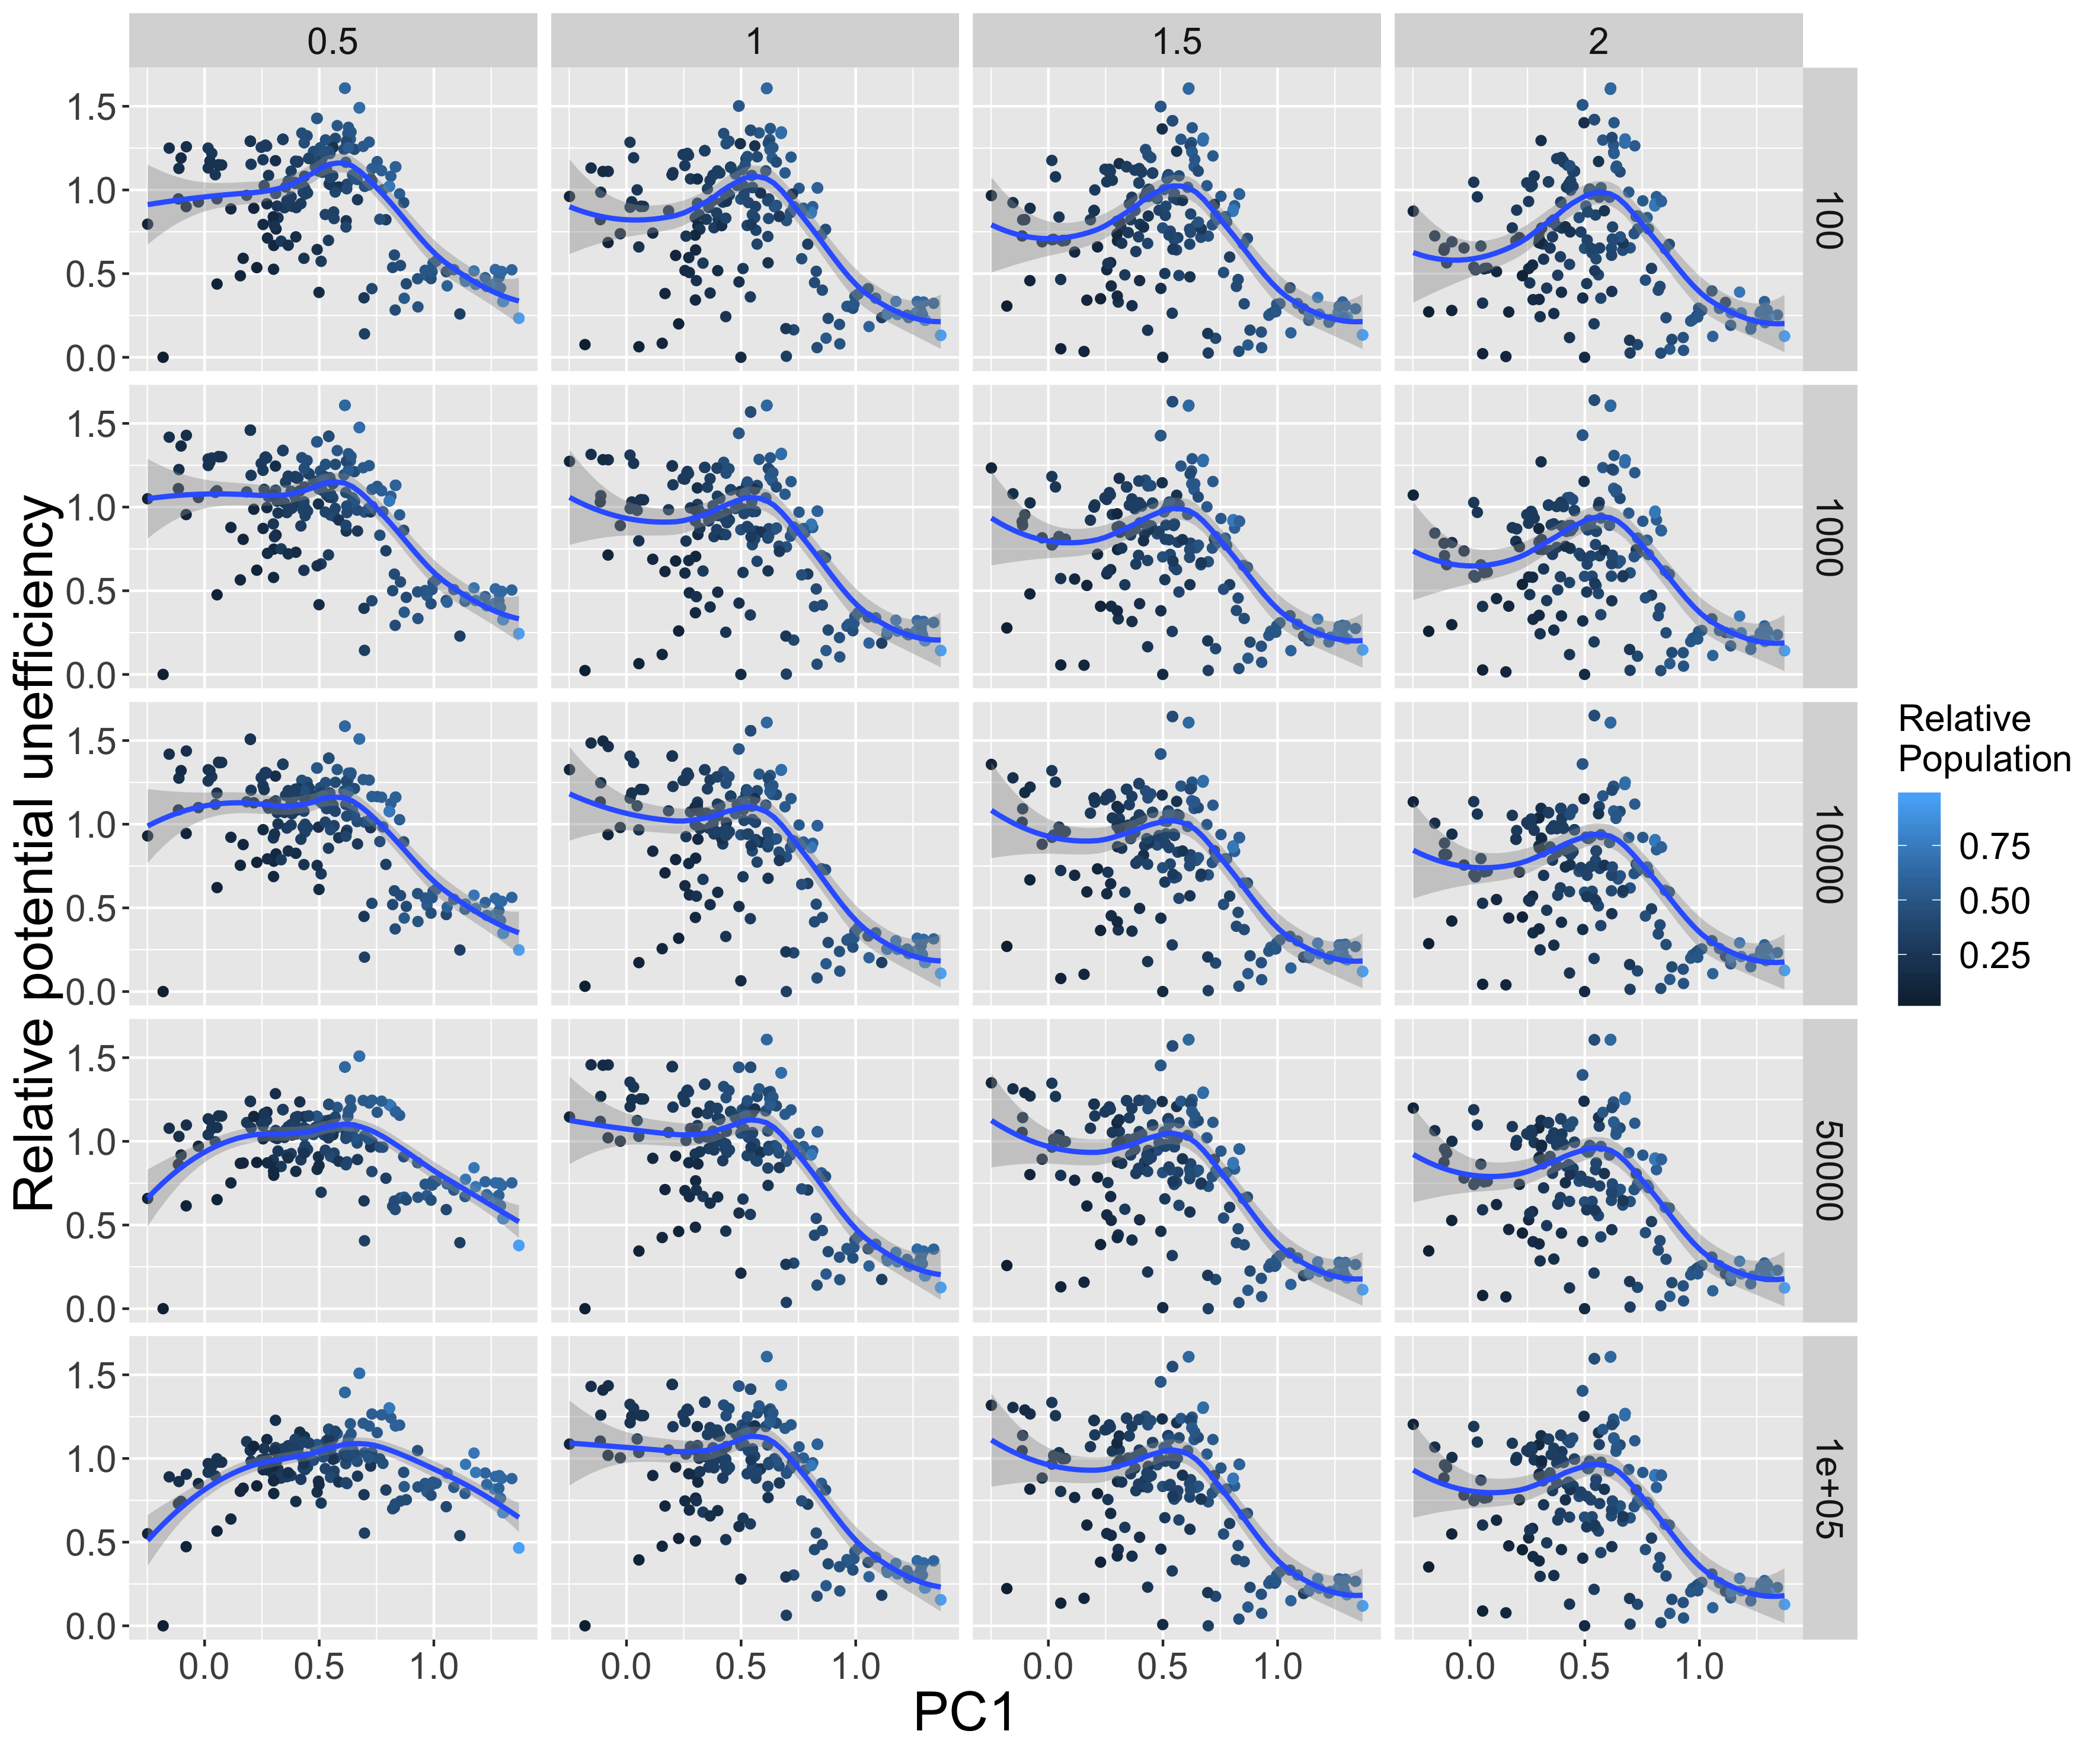
\includegraphics[width=0.49\textwidth]{figures/aggreg_morpho_pc1-relefficiency.png}
%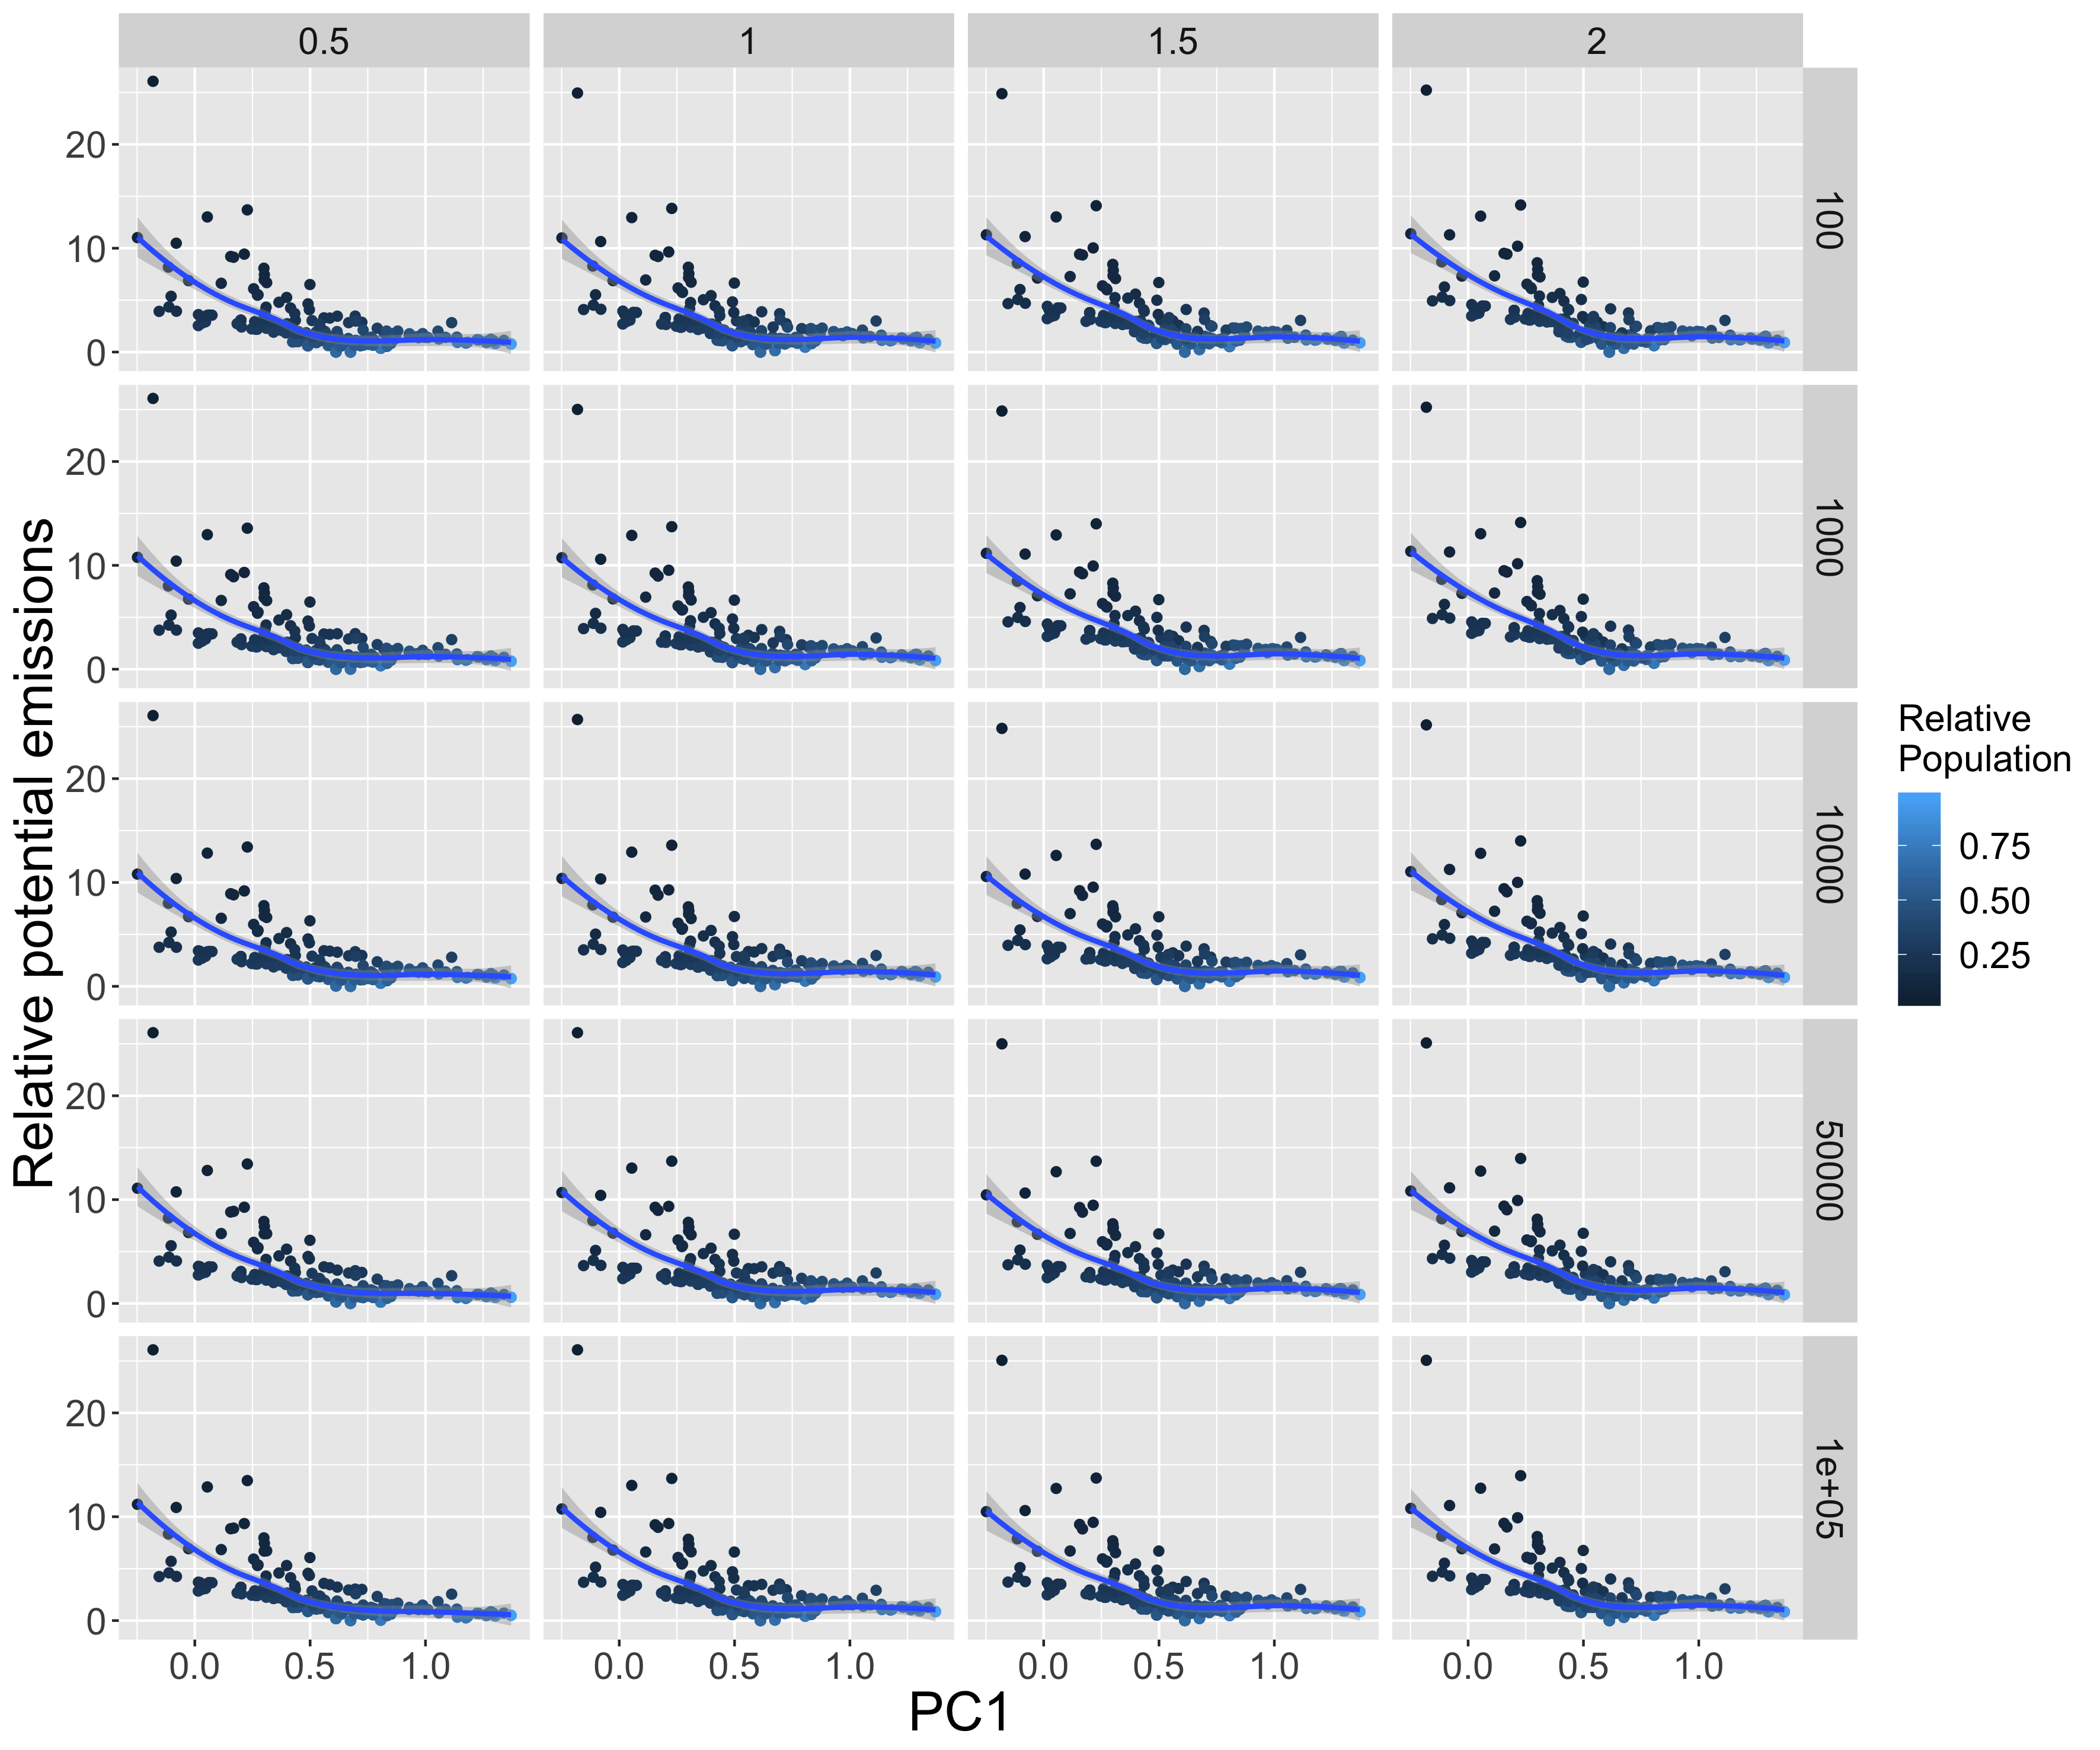
\includegraphics[width=0.49\textwidth]{figures/aggreg_morpho_pc1-relemissions.png}

% TODO : curves for emissions rescale to the same -> link with Caruso profiles ? ; investigate that, and why not for efficiency.





%\section{Acknowledgment}
%

%\section{Biography}
%Here, feel free to add short biographies of the authors.






\end{document}





%%%%%%%%
%% -- TEMPLATES

%\begin{table}
%  \newcolumntype{+}{>{\global\let\currentrowstyle\relax}}
%  \newcolumntype{^}{>{\currentrowstyle}}
%  \newcommand{\rowstyle}[1]{\gdef\currentrowstyle{#1}%
%    #1\ignorespaces
%  }
%  \centering
%  \begin{tabular}{+>{\bfseries}l^c^c^c^c}
%    \hline
%    \rowstyle{\bfseries}
%    & Sepal.Length & Sepal.Width & Petal.Length & Petal.Width\\
%    Setosa & 5.006 & 3.428 & 1.462 & 0.246\\
%    Versicolor & 5.936 & 2.77  & 4.26  & 1.326\\
%    Verginica & 6.588 & 2.974 & 5.552 & 2.026\\
%    \hline
%  \end{tabular}
%  \caption{Morbi malesuada diam at magna condimentum.}
%  \label{tab:example}
%\end{table}

%
%\begin{figure*}[ht] 
%\resizebox{10cm}{7cm}
%  {\includegraphics[width=11cm]{spider.jpg}}
%  \centering
%  \label{frog}
%  \caption{A spider, Picture from Didier Josselin.}
%  \end{figure*}
%  


